\documentclass[a4paper,10pt,fleqn]{ltjsarticle} % fleqn:数式を左揃えにする

\input{/home/yorit/study/.util/latex_preamble/Preamble}

\usepackage{subfiles}

\newcommand{\ii}{\mathrm{i}}
\newcommand{\jj}{\mathrm{j}}
\newcommand{\ee}{\mathrm{e}}
\renewcommand{\abs}[1]{\lvert #1 \rvert}
\DeclareSIUnit{\vpp}{\ensuremath{\mathrm{V_{pp}}}}

% siunitx で数式を扱う
\newcommand{\SIeq}[2]{\SI[parse-numbers=false, per-mode=symbol]{#1}{#2}}
\newcommand{\sis}[1]{\si[per-mode=symbol]{#1}}
\newcommand{\SIs}[2]{\SI[per-mode=symbol]{#1}{#2}}

\graphicspath{{../figures/}}

\coursetitle{電気電子工学実習}
\title{電気電子工学実習報告書}
\subtitle{太陽光発電を利用した電源システム設計}
\department{工学部電気電子工学科}
\id{1026351380}
\author{5班 市川弦慈}
\date{\today}


\begin{document}
\maketitle
\thispagestyle{empty}

\newpage
\setcounter{page}{1}

\section{概要}

本実習では、環境によって出力の異なる太陽光電池を用いて安定した電源供給システムを構築し、またそのシステムを評価する。

% % !TEX root = 1_power_supply.tex
\documentclass[1_power_supply.tex]{subfiles}
\graphicspath{{../figures/}}
\begin{document}

\section{太陽電池の特性}

  \subsection{目的}

    \begin{enumerate}
      \item 照度と,光源からの距離との関係を調べる.
      \item 太陽電池の特性を測定し,等価回路のパラメータや出力できる電力について評価する.
    \end{enumerate}

  \subsection{原理}

    今回作成するシステムの入口となる光エネルギーから電気エネルギーへの変換部分を担うのが太陽電池であり,これは,ダイオードの光特性を利用した素子である.太陽電池の等価回路は図\ref{fig:1_2}の青点線部で表される.このとき図\ref{fig:1_2}中の$V,I$に関して,
    \begin{align}
      I = I_\mathrm{ph}-I_0\left\{\exp[\frac{e(V+R_\mathrm{s}I)}{nkT}-1]\right\}-\frac{V+R_\mathrm{s}I}{R_\mathrm{sh}}
    \end{align}

    という関係が成り立つ.ここで,$I_0$ :飽和電流,$e$ :電気素量,$k$ :ボルツマン定数,$n$ :接合定数,$T$ :絶対温度,$I_\mathrm{ph}$ :光電流である.


    \begin{figure}[htbp]
      \begin{center}
        \scalebox{0.1}{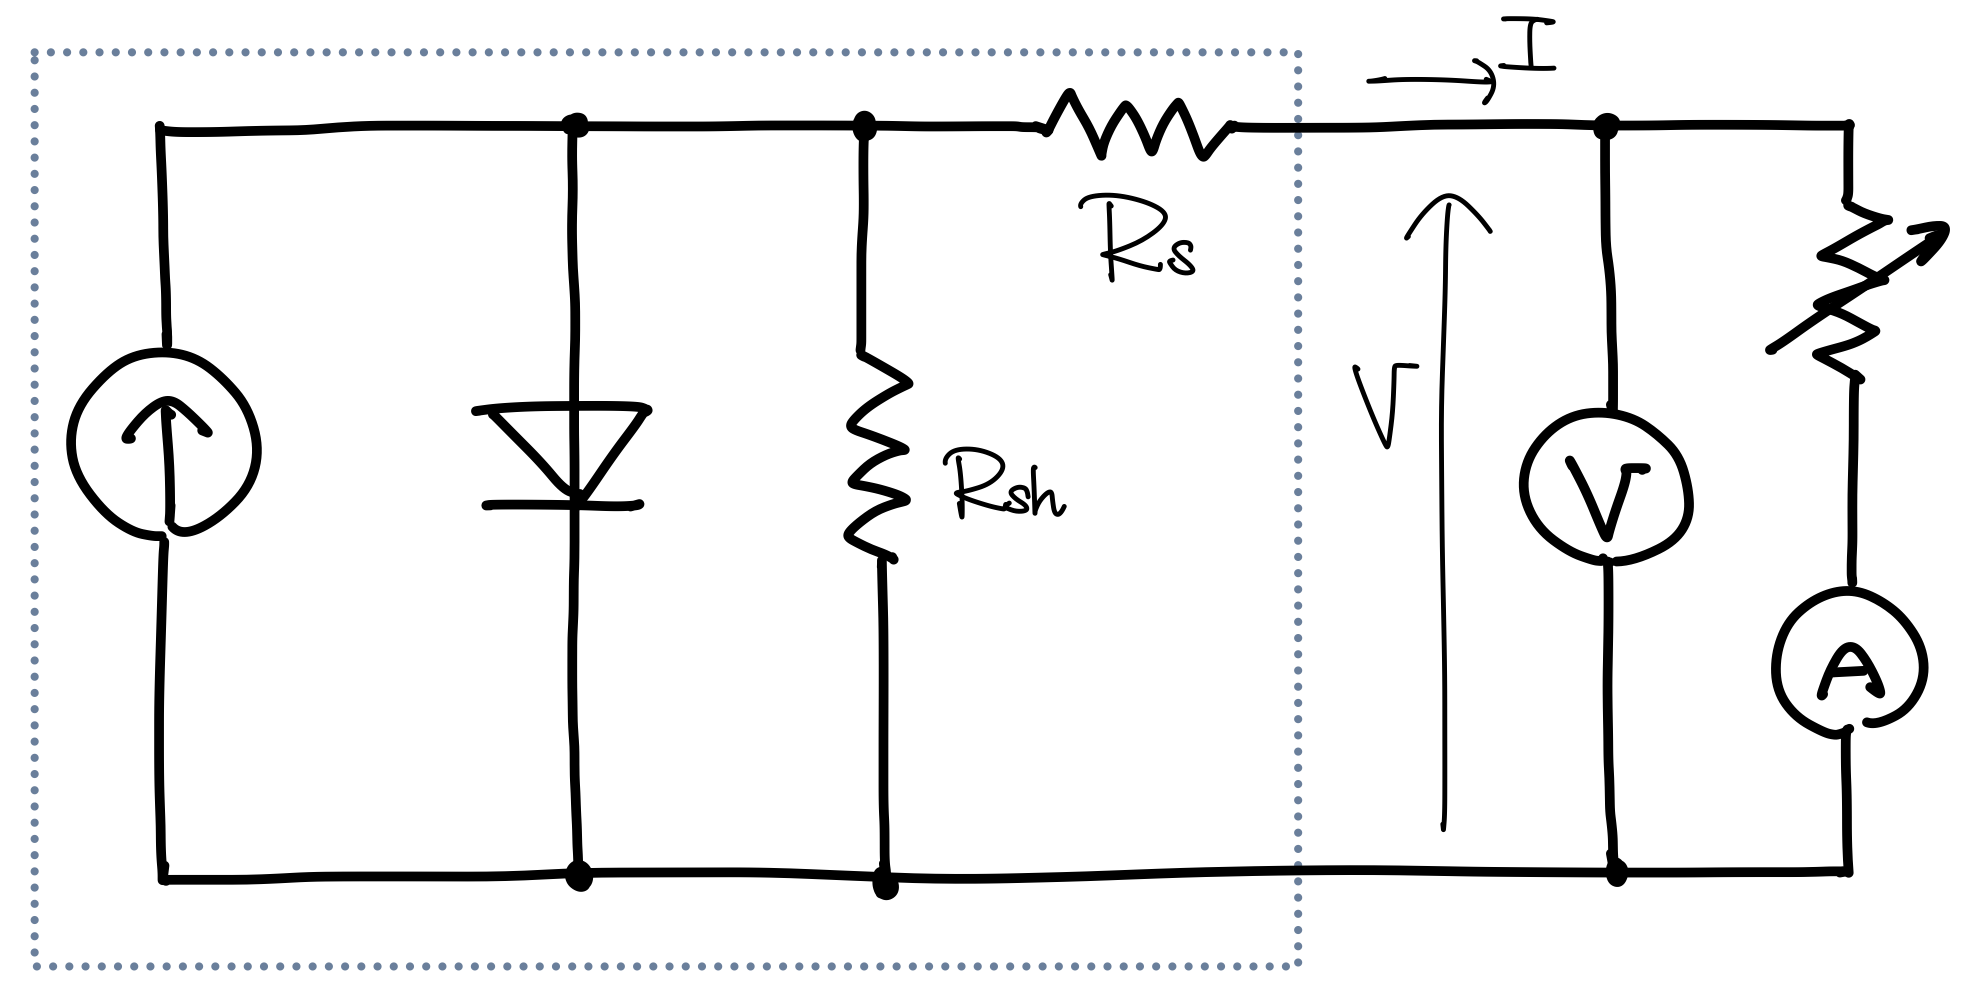
\includegraphics{1_2.png}}
        \caption{太陽電池の特性を測定するための回路}\label{fig:1_2}
      \end{center}
    \end{figure}

    等価回路の抵抗を求める際は,ダイオードが動作している(電圧源とみなせる)ときと,動作していない(開放とみなせる)ときに分けて考える.

    \subsubsection{ダイオードが動作しているとき}

      ダイオードの動作電圧を$V_\mathrm{on}$とすると,キルヒホッフの電圧則から,

      \begin{align}
        V_\mathrm{on} = V+R_\mathrm{s}I
      \end{align}

      両辺を$V$で微分して,

      \begin{align}
        0            &= 1+R_\mathrm{s}\dv{I}{V}  \\
        R_\mathrm{s} &= \left.- \dv{V}{I}\right|_{V\sim V_\mathrm{on}} \label{eq:R_s}
      \end{align}

      となる.

    \subsubsection{ダイオードが動作していないとき}

      キルヒホッフの電圧則から,

      \begin{align}
        V+R_\mathrm{s}I = R_\mathrm{sh}(I_\mathrm{ph}-I)
      \end{align}

      両辺を$I$で微分して,

      \begin{align}
        \dv{V}{I}+R_\mathrm{s} &= -R_\mathrm{sh}  \\
        R_\mathrm{sh}          &= \left.-\dv{V}{I}\right|_{V\sim 0}-R_\mathrm{s} \label{eq:R_sh}
      \end{align}

  \subsection{方法}

    \subsubsection{照度と光源からの距離に関する実験(実験1.1)}


      \begin{figure}[htbp]
        \begin{center}
          \scalebox{0.2}{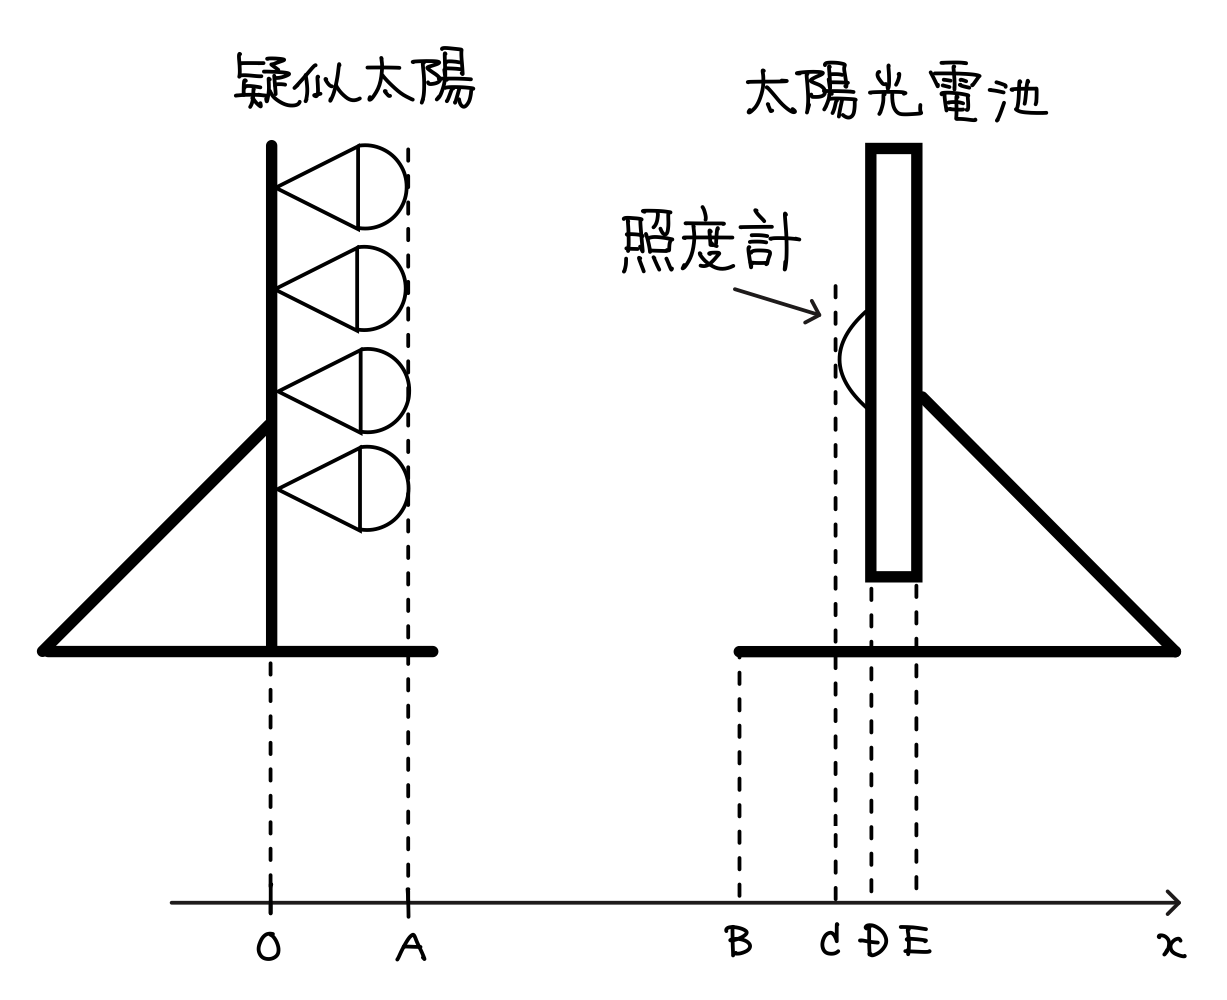
\includegraphics{1_1.png}}
          \caption{照度測定の様子を横から見た図}\label{fig:1_1}
        \end{center}
      \end{figure}

      図\ref{fig:1_1}のように擬似太陽と太陽光電池,照度計を配置し,疑似太陽と太陽光電池との間隔を変えて,太陽光電池の中央での照度を計測した.測定点は$\mathrm{OB}=\SIs{60}{\centi\meter},\SIs{75}{\centi\meter},\SIs{90}{\centi\meter},\SIs{105}{\centi\meter},\SIs{120}{\centi\meter}$の5点とした.
      % なお,距離の測定は図\ref{fig:1_1}中OB間で行い,適切な変換でもってAC間の距離を導出した.測定した間隔は,OB間が$\SIs{60}{\centi\meter},\SIs{75}{\centi\meter},\SIs{90}{\centi\meter},\SIs{105}{\centi\meter},\SIs{120}{\centi\meter}$の5つの場合である.

    \subsubsection{太陽電池の特性を調べる実験(実験1.2)}


      \begin{figure}[htbp]
        \begin{center}
          \scalebox{0.11}{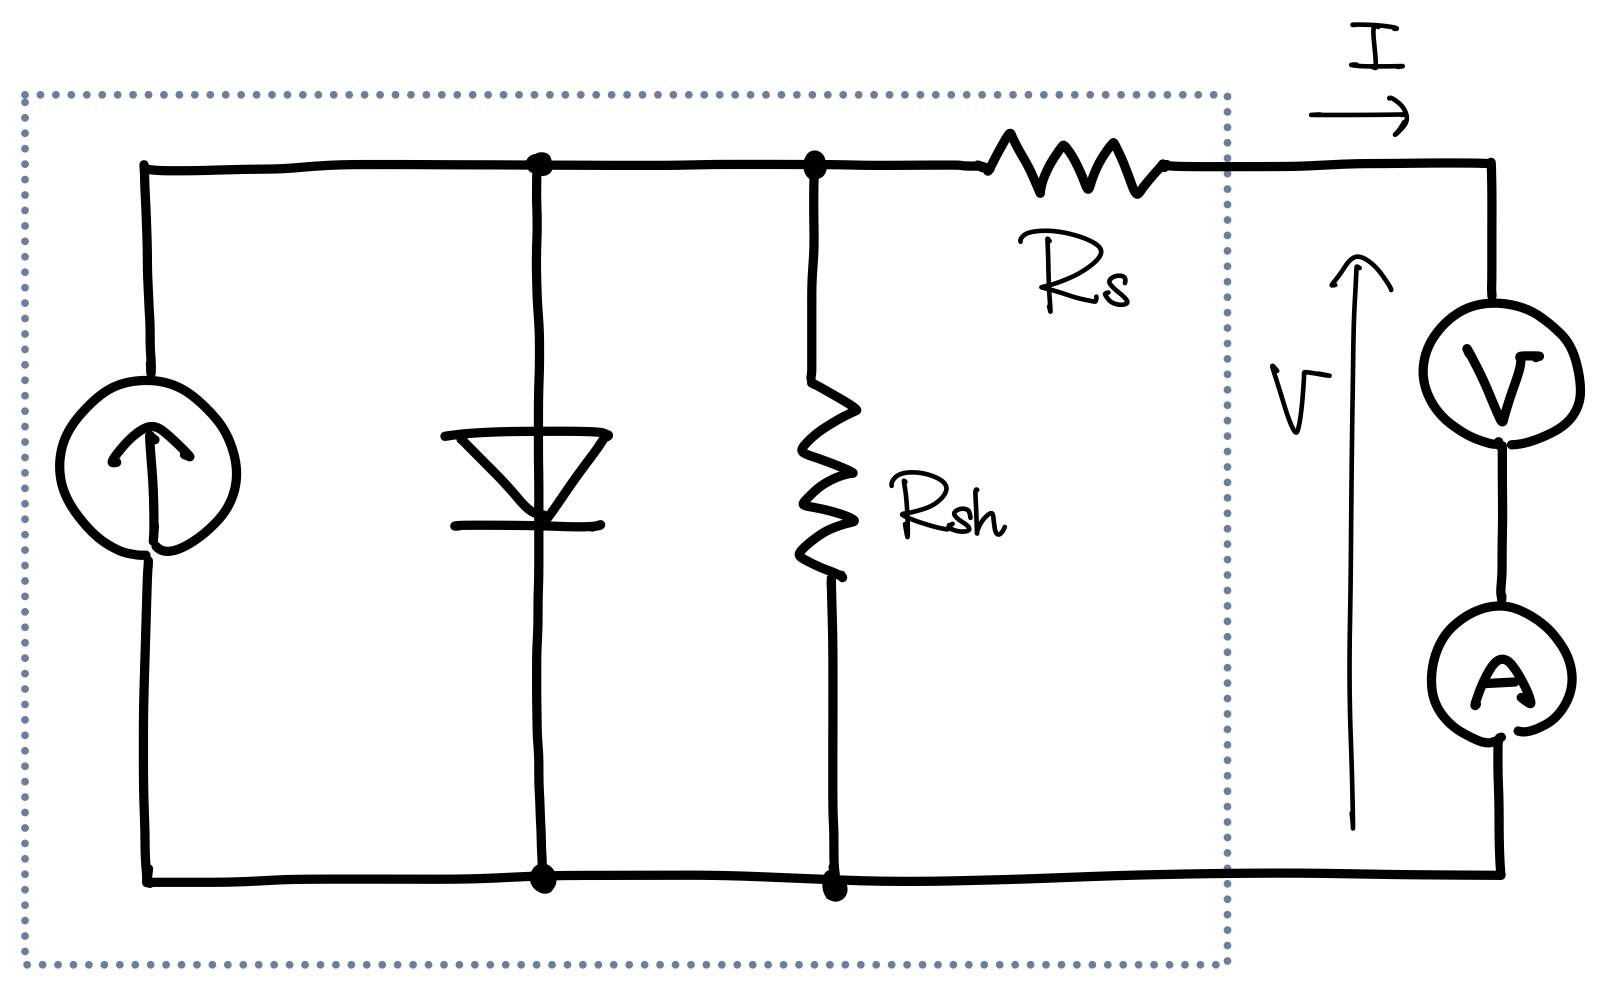
\includegraphics{1_3.png}}
          \caption{太陽電池の特性を測定するための回路($I$が$\SIs{0}{\ampere}$近傍のとき)}\label{fig:1_3}
        \end{center}
      \end{figure}

      図\ref{fig:1_1}中OB間の距離が$\SIs{60}{\centi\meter},\SIs{105}{\centi\meter},\SIs{120}{\centi\meter}$の3つの場合について,図\ref{fig:1_2}の回路を用いて$V,I$を測定した.また,$I$が$\SIs{0}{\ampere}$近傍の測定については,抵抗を印加しない開放での測定を再現するため,図\ref{fig:1_3}の回路を用いた.

  \subsection{使用器具}
    (型番を記していない器具については確認し次第追記します.)
    \begin{enumerate}
      \item 太陽電池モジュール : 昭和ソーラーエネルギー(株) GT234
      \item 電圧計
      \item 電流計
    \end{enumerate}

  \subsection{結果}

    \subsubsection{実験1.1}

      $\mathrm{AC}=\mathrm{OB}-\SIs{4.5}{\centi\meter}$と照度の測定結果を図\ref{fig:1_dE}に示す.


      \begin{figure}[htbp]
        \begin{center}
          \scalebox{0.5}{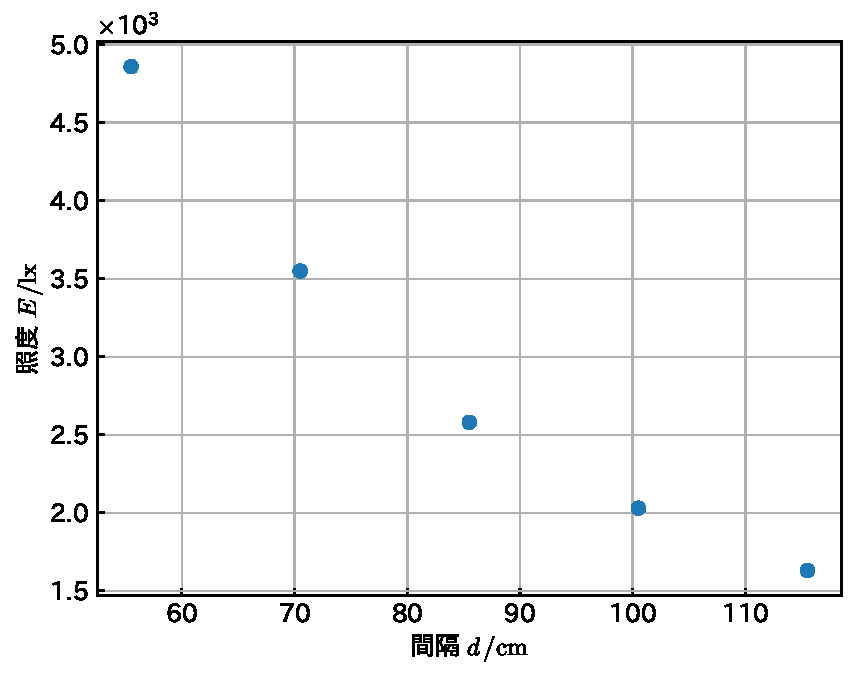
\includegraphics{1_dE.pdf}}
          \caption{光源から照度計までの距離と照度との関係}\label{fig:1_dE}
        \end{center}
      \end{figure}

    \subsubsection{実験1.2}

      各間隔での電流電圧特性の測定結果を図\ref{fig:1_VI}に示す.


      \begin{figure}[htbp]
        \begin{center}
          \scalebox{0.75}{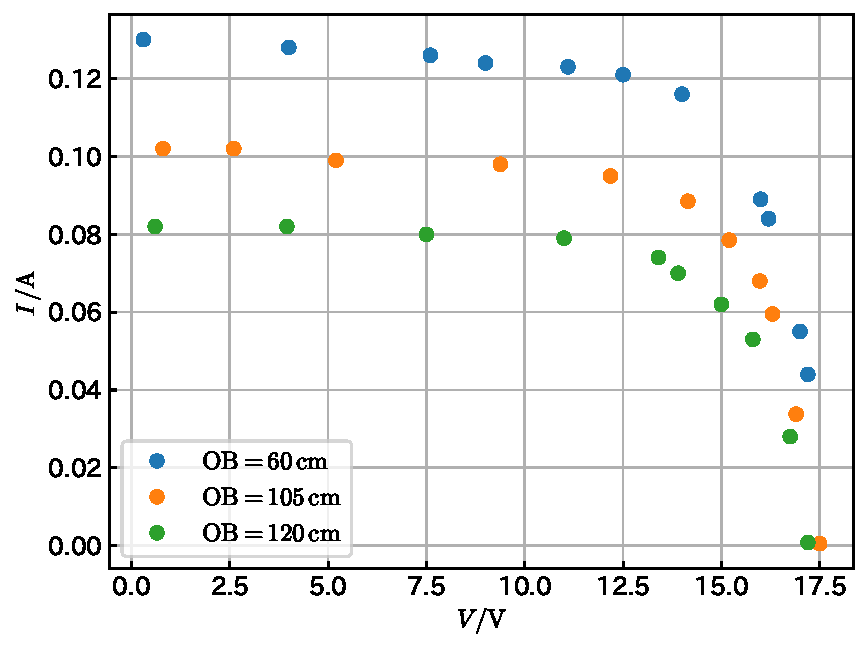
\includegraphics{1_VI.pdf}}
          \caption{光を照射したときの太陽電池の電流電圧特性の測定結果}\label{fig:1_VI}
        \end{center}
      \end{figure}

  \subsection{考察}

    \subsubsection{実験1.1}

      光源が点光源の場合は,照度は距離の逆二乗に比例することが知られている.今回の実験では点光源ではないことを考慮し,照度を$E$,距離を$d$とおいて,

      \begin{align}
        E = \frac{A}{ad^2+bd+c}
      \end{align}

      に従うことを仮定する.$A,a,b,c$は定数である.図\ref{fig:1_dE}に対しフィッティングを行ったものを図\ref{fig:1_dE_fit}に示す.


      \begin{figure}[htbp]
        \begin{center}
          \scalebox{0.5}{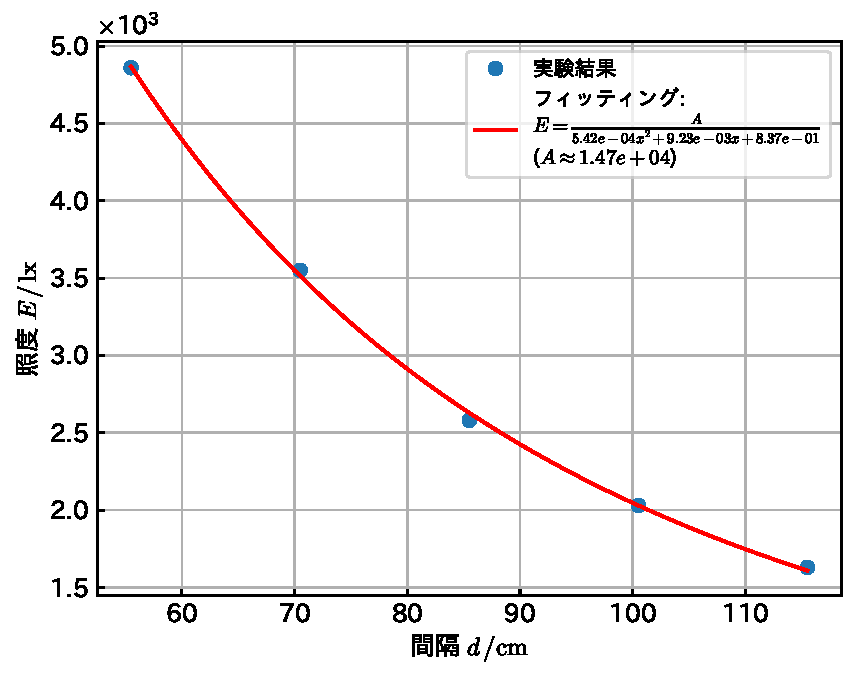
\includegraphics{1_dE_fit.pdf}}
          \caption{照度測定結果とそのフィッティング}\label{fig:1_dE_fit}
        \end{center}
      \end{figure}

      今回の測定から,

      \begin{align}
        E = \frac{\SIs{1.47e4}{\lumen}}{(\num{5.4e-4})\times d^2+(\SIs{9.2e-3}{\meter})\times d+(\SIs{0.84}{\meter^2})}
      \end{align}

      と係数を決定できた.

    \subsubsection{実験1.2}

      代表として$\mathrm{OB}=\SIs{105}{\centi\meter}$の場合について解析する.


      \begin{figure}[htbp]
        \begin{center}
          \scalebox{0.5}{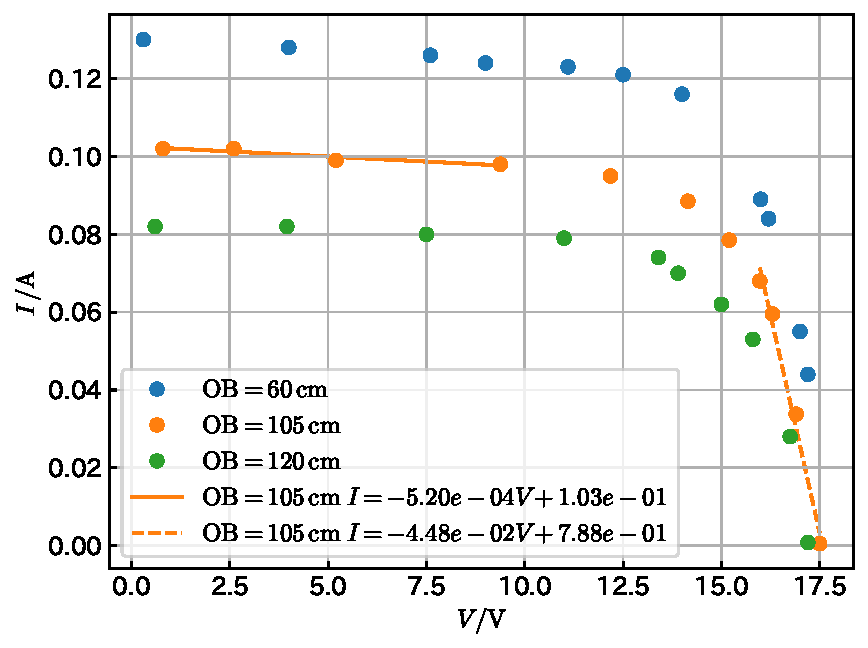
\includegraphics{1_VI_fit.pdf}}
          \caption{電流電圧特性の測定結果とフィッティング}\label{fig:1_VI_fit}
        \end{center}
      \end{figure}

      ダイオードが動作している領域・動作していない領域でフィッティングした図を図\ref{fig:1_VI_fit}に示す.ここで得られた傾きと式(\ref{eq:R_s})(\ref{eq:R_sh})から,

      \begin{align}
        \SIeq{R_\mathrm{s}}{\per\ohm}  &=      -\frac{1}{\num{-4.48e-2}}  \\
        R_\mathrm{s}                   &\simeq \SIs{22.3}{\ohm}  \\
        \SIeq{R_\mathrm{sh}}{\per\ohm} &=      -\frac{1}{\num{-5.20e-4}}-22.3  \\
        R_\mathrm{sh}                  &\simeq \SIs{1.90e3}{\ohm}
      \end{align}

      と,等価回路の抵抗値が得られる.

% % !TEX root = 1_power_supply.tex
\documentclass[1_power_supply.tex]{subfiles}
\graphicspath{{../figures/}}
\begin{document}

\section{DC-DCコンバータ}

\subsection{目的}

太陽電池から得られる直流の電圧,電流を増幅するためにDC-DCコンバータ農地,チュックコンバータを用いる.本実験では,チュックコンバータのスイッチ制御を変化させたときの電力利得を調べる.

\subsection{原理}

DC-DCコンバータは,スイッチングを行うことで電圧を増幅できる装置である.1周期のスイッチングの中でのオンの時間の割合(デューティ比 $D$)によって,入力電圧$V_\mathrm{i}$と出力電圧$V_\mathrm{o}$との間に
\begin{align}
	V_\mathrm{o} = -\frac{D}{1-D}V_\mathrm{i}
\end{align}

という関係が成り立つ.

\subsection{方法}

\begin{figure}[htbp]
	\begin{center}
		\scalebox{0.1}{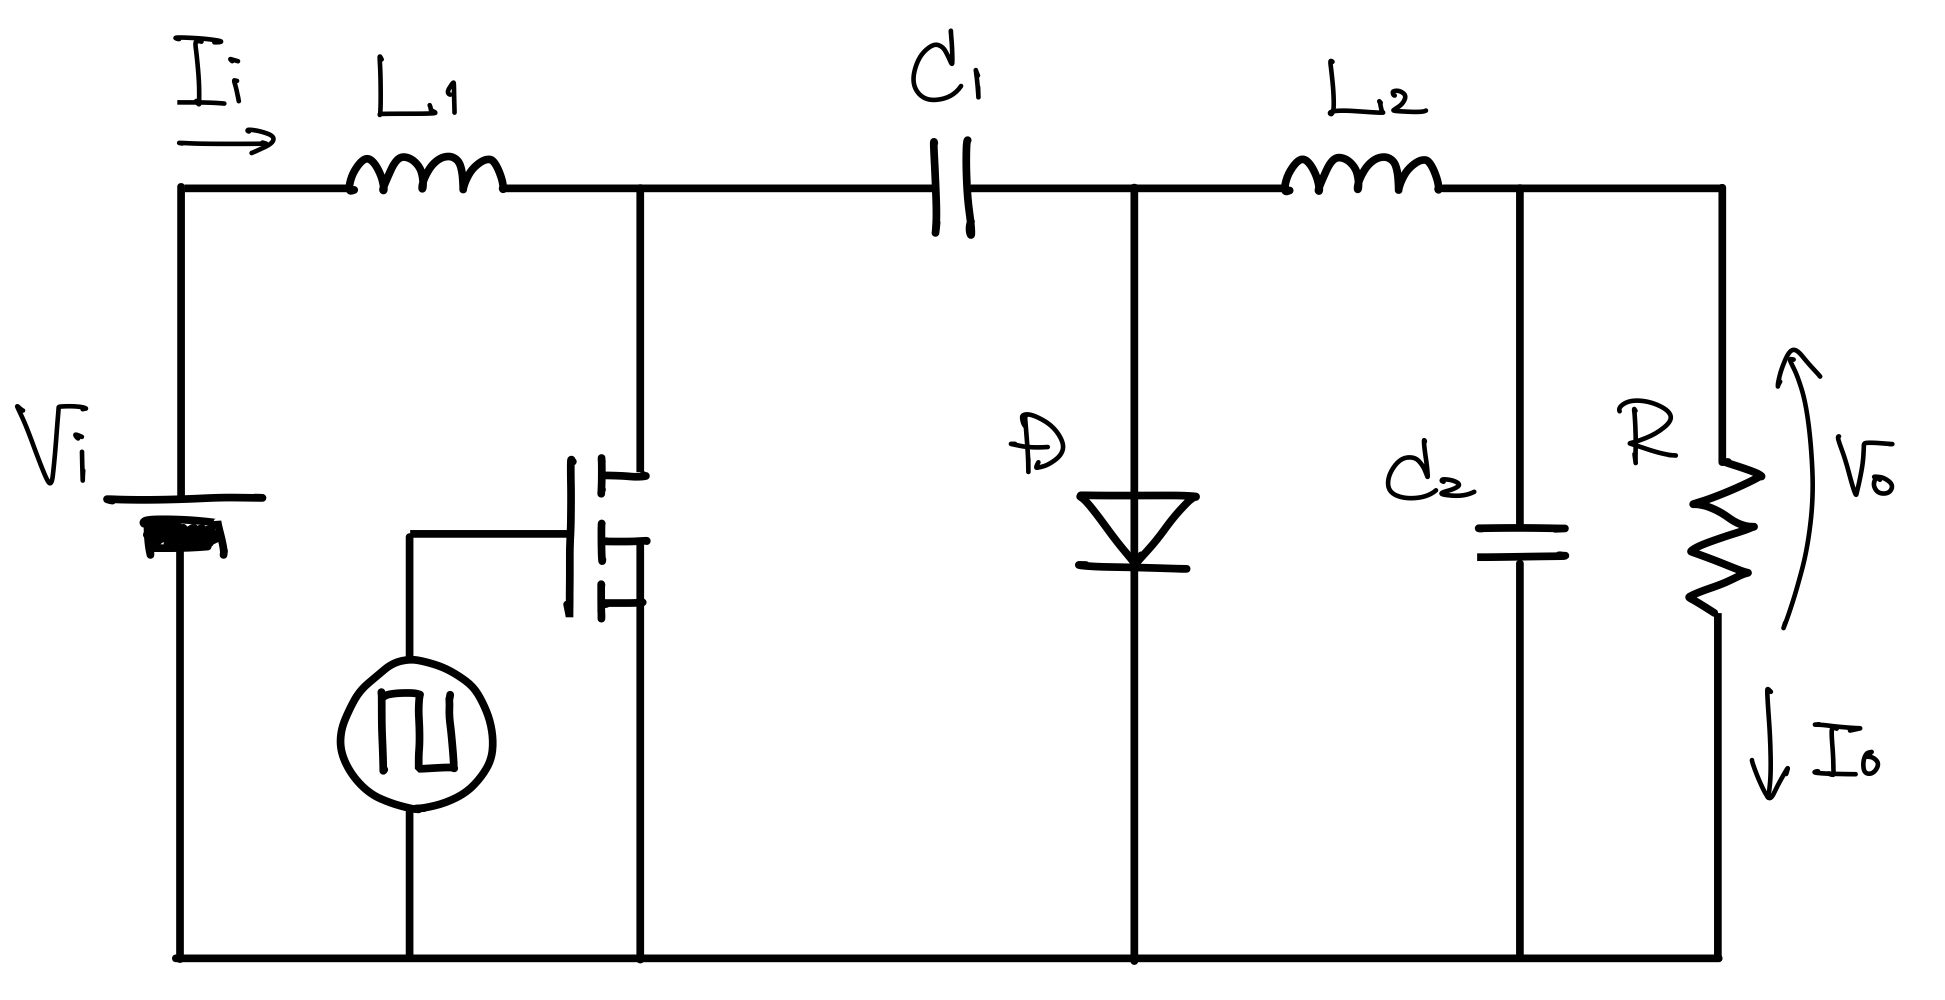
\includegraphics{1_4.png}}
		\caption{測定対象の回路}\label{fig:1_4}
	\end{center}
\end{figure}

測定対象の回路を図\ref{fig:1_4}に示す.この回路に対して,方形波にデューティ比がそれぞれ \\$\SIs{10}{\percent},\SIs{25}{\percent},\SIs{40}{\percent},\SIs{50}{\percent},\SIs{60}{\percent},\SIs{75}{\percent},\SIs{80}{\percent}$を印加したときの入力電圧$V_\mathrm{i}$,入力電流$I_\mathrm{i}$,出力電圧$V_\mathrm{o}$,出力電流$I_\mathrm{o}$を測定し,入力電力$P_\mathrm{i}$と出力電力$P_\mathrm{o}$の関係をプロットする.
	各素子や信号の詳細は,
	\begin{enumerate}
		\item $L_1=\SIs{470}{\text{\textmu}\henry}$ % \micro が使えなかったのでやむを得ず
		\item $L_2=\SIs{470}{\text{\textmu}\henry}$
		\item $C_1=\SIs{100}{\text{\textmu}\farad}$
		\item $C_2=\SIs{100}{\text{\textmu}\farad}$
		\item 方形波 : (周波数 : $\SIs{100}{kHz}$, 電圧 : $\SIs{5}{\vpp}$, オフセット : $\SIs{2.5}{\volt}$)
	\end{enumerate}
	である.

	\subsection{使用器具}

	(型番については確認し次第追記します.)
	\begin{enumerate}
		\item 電圧計
		\item 電流計
		\item 直流電源
		\item ファンクションジェネレータ
	\end{enumerate}

	\subsection{結果}

	各デューティ比$D$での電力利得を図\ref{fig:2_10p},\ref{fig:2_25p},\ref{fig:2_40p},\ref{fig:2_50p},\ref{fig:2_60p},\ref{fig:2_75p},\ref{fig:2_80p},に示す.

	\begin{figure}[htbp]
		\begin{minipage}{0.45\columnwidth}
			\centering
			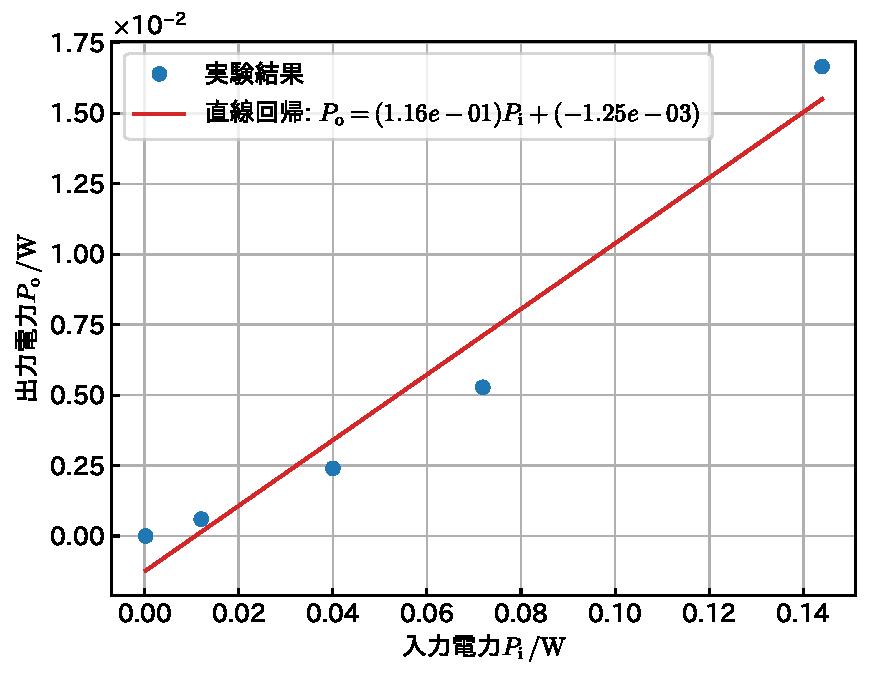
\includegraphics[width=0.8\columnwidth]{2_10p.pdf}
			\caption{$D=0.1$}\label{fig:2_10p}
		\end{minipage}
		\begin{minipage}{0.45\columnwidth}
			\centering
			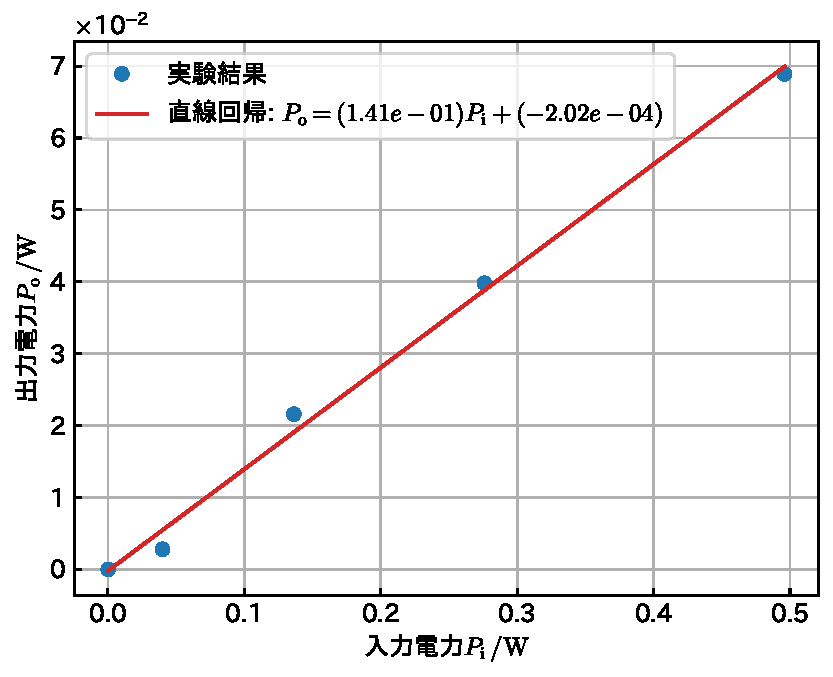
\includegraphics[width=0.8\columnwidth]{2_25p.pdf}
			\caption{$D=0.25$}\label{fig:2_25p}
		\end{minipage}

		\vspace{1.5mm}
		\begin{minipage}{0.45\columnwidth}
			\centering
			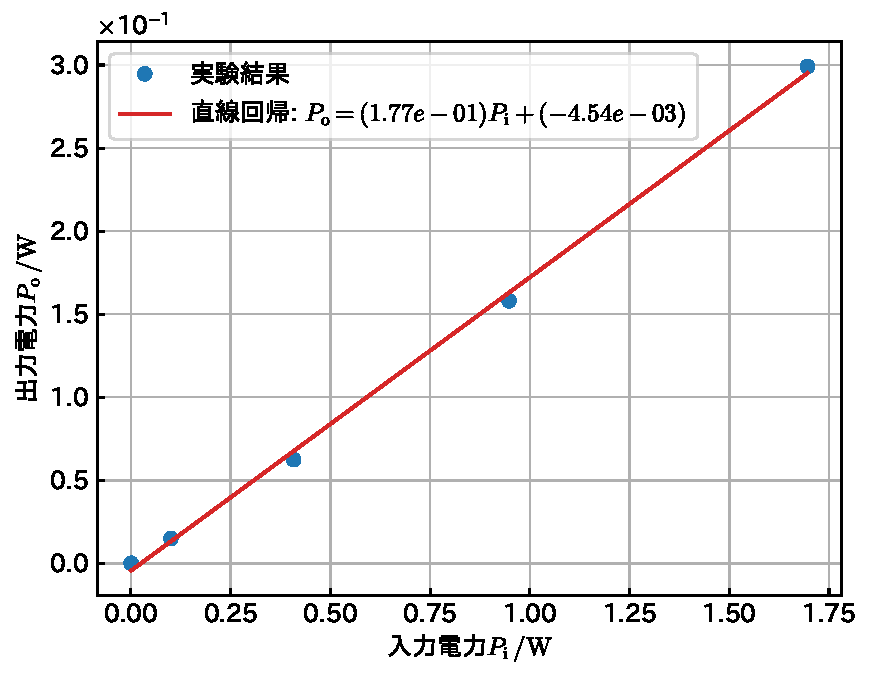
\includegraphics[width=0.8\columnwidth]{2_40p.pdf}
			\caption{$D=0.4$}\label{fig:2_40p}
		\end{minipage}
		\begin{minipage}{0.45\columnwidth}
			\centering
			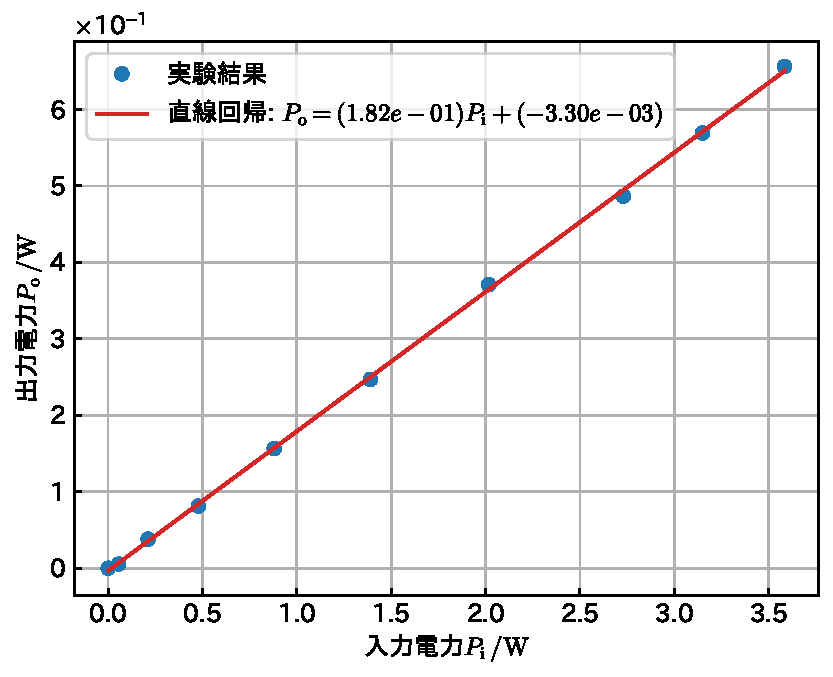
\includegraphics[width=0.8\columnwidth]{2_50p.pdf}
			\caption{$D=0.5$}\label{fig:2_50p}
		\end{minipage}

		\vspace{1.5mm}
		\begin{minipage}{0.45\columnwidth}
			\centering
			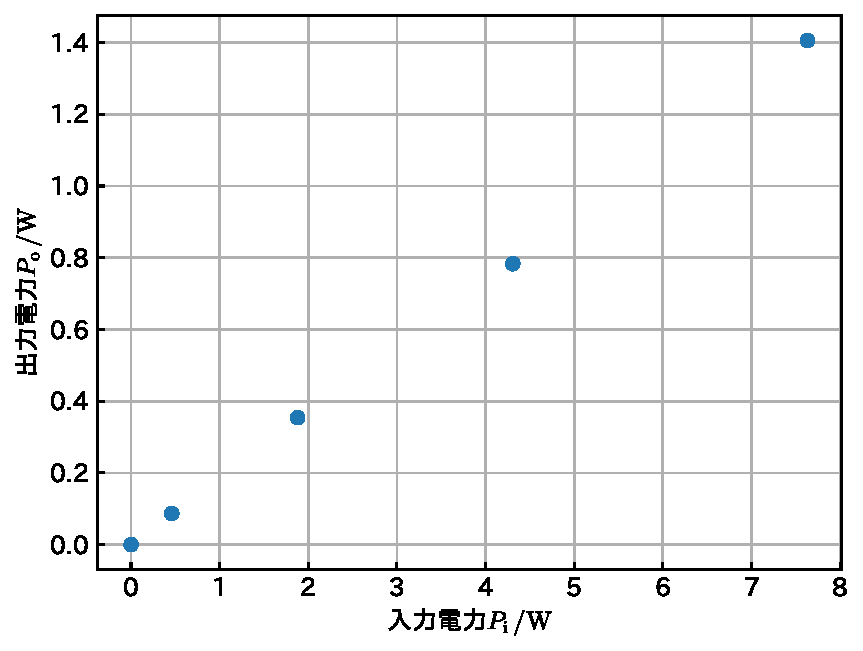
\includegraphics[width=0.8\columnwidth]{2_60p.pdf}
			\caption{$D=0.6$}\label{fig:2_60p}
		\end{minipage}
		\begin{minipage}{0.45\columnwidth}
			\centering
			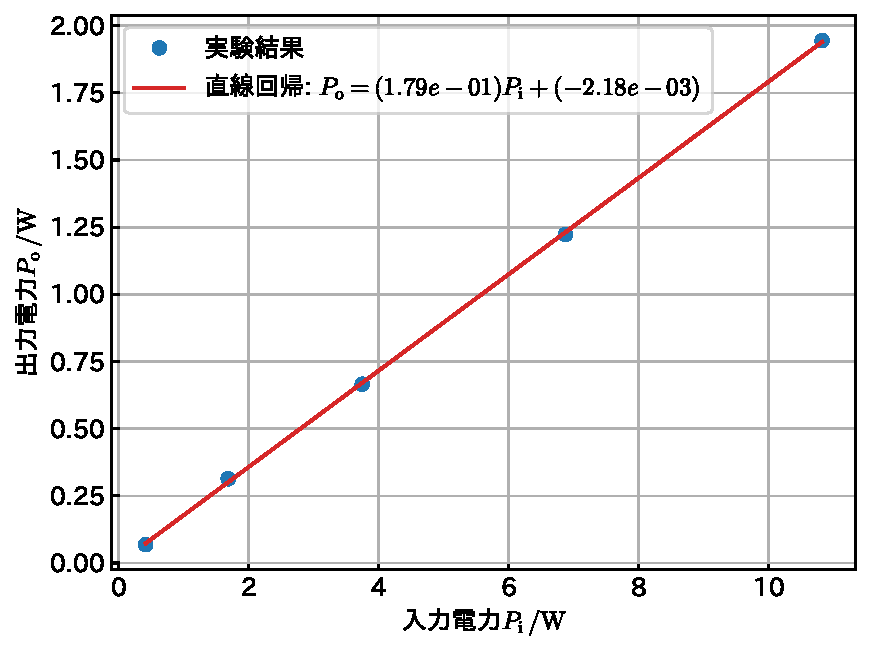
\includegraphics[width=0.8\columnwidth]{2_75p.pdf}
			\caption{$D=0.75$}\label{fig:2_75p}
		\end{minipage}

		\vspace{1.5mm}
		\begin{minipage}{0.45\columnwidth}
			\centering
			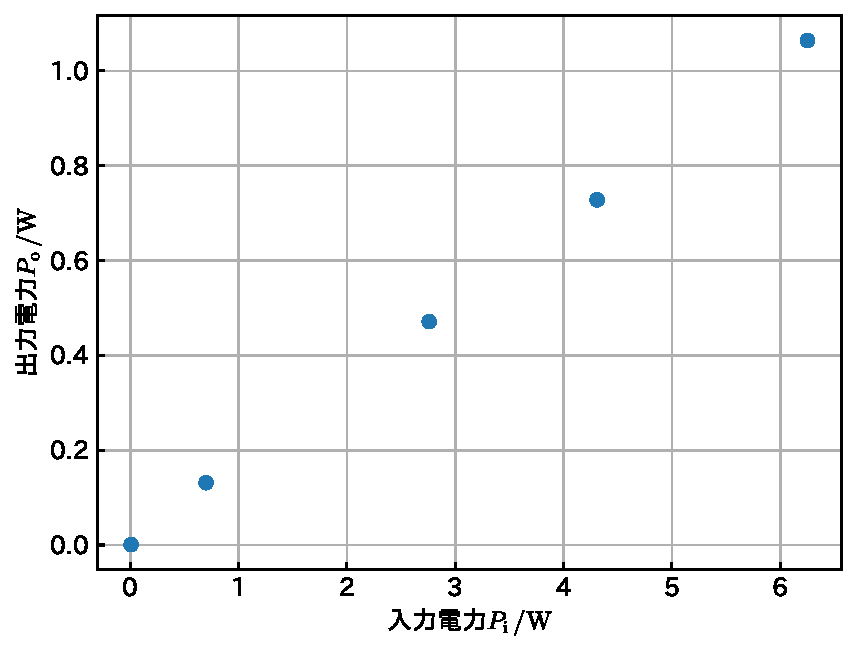
\includegraphics[width=0.8\columnwidth]{2_80p.pdf}
			\caption{$D=0.8$}\label{fig:2_80p}
		\end{minipage}
		\begin{minipage}{0.45\columnwidth}
			\centering
			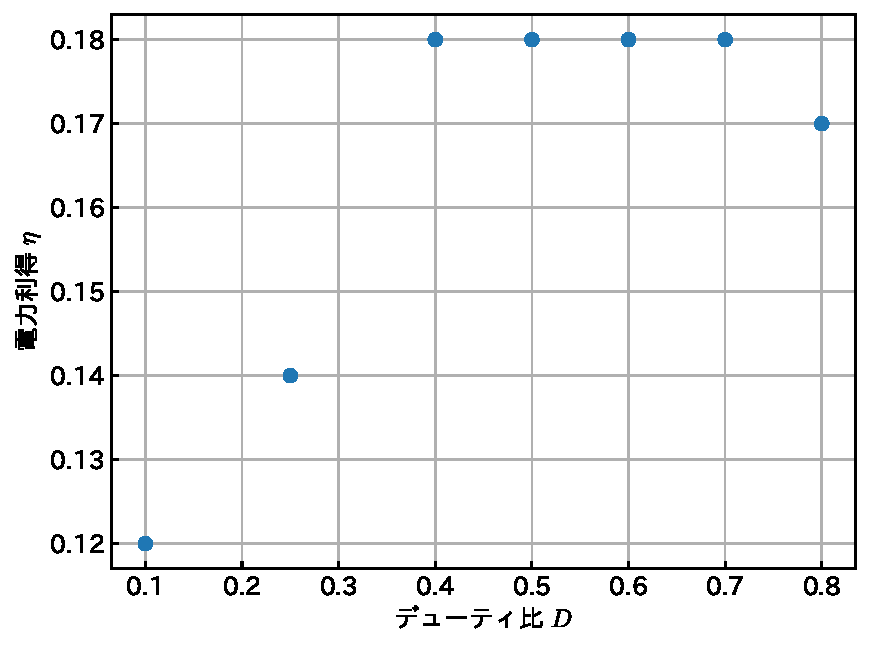
\includegraphics[width=0.8\columnwidth]{2_d_eta.pdf}
			\caption{デューティ比と電力利得の関係}\label{fig:2_d_eta}
		\end{minipage}
	\end{figure}

	\subsection{考察}

	デューティ比と電力利得の関係を表すプロットを図\ref{fig:2_d_eta}に示す.この関係から,電力利得を良くするためにはデューティ比が$0.4\sim 0.7$の範囲で動作させればいいことがわかる.

% %!TEX root = 1_power_supply.tex
\documentclass[1_power_supply.tex]{subfiles}
\graphicpath{{../figures}}
\begin{document}

\section{DCDCコンバータへのフィードバック回路}

  \subsection{目的}

    DCDCコンバータの出力を制御するためのフィードバック回路を導入し,その回路の入出力特性と,フィードバック付きDCDCコンバータの入出力特性について調べる.

  \subsection{原理}

    DCDCコンバータの出力を一定にするためにフィードバック回路を考える.DCDCコンバータの制御はデューティ比の異なる方形波で行うので,フィードバック回路の出力は方形波である必要がある.この要件を満たすため,フィードバック回路は,DCDCコンバータの出力と目標電圧との差信号を出力する回路と,その差と三角波を比較する回路を接続するものにする.

    \subsubsection{差信号を生成する回路}

      DCDCコンバータからの出力が負であるから,差信号を生成するためには出力電圧と目標電圧との和を取ればよい.加算回路を図\ref{fig:3_add}に示す.加算器の原理から,

      \begin{align}
        V_\mathrm{e} &= -\frac{R_\mathrm{f}}{R_0}(V_\mathrm{ref} + V_\mathrm{in})  \\
                     &= -\frac{R_\mathrm{f}}{R_0}(V_\mathrm{ref} - |V_\mathrm{in}|)
      \end{align}
      という関係が成り立つ.ここで,$K_\mathrm{fb} \coloneq -R_\mathrm{f}/R_0$とすると関係式は,

      \begin{equation}
        V_\mathrm{e} = K_\mathrm{fb}(V_\mathrm{ref} - |V_\mathrm{in}|)
      \end{equation}
      と書き直せる.

    \subsubsection{比較器}

      今回の実験では図\ref{fig:3_comp}で表される回路で方形波を出力する.直流電源と三角波の電圧を比較することで,様々なデューティ比の方形波が出力できる.ここで,三角波の振幅をpeak-to-peakで$V_\mathrm{tri}$とすると,方形波のデューティ比$D$は,

      \begin{equation}
        D = \frac{1}{2}-\frac{V_\mathrm{e}}{V_\mathrm{tri}} \label{eq:D}
      \end{equation}
      と計算することができる.


      \begin{figure}[htbp]
        \begin{minipage}{0.45\columnwidth}
          \centering
          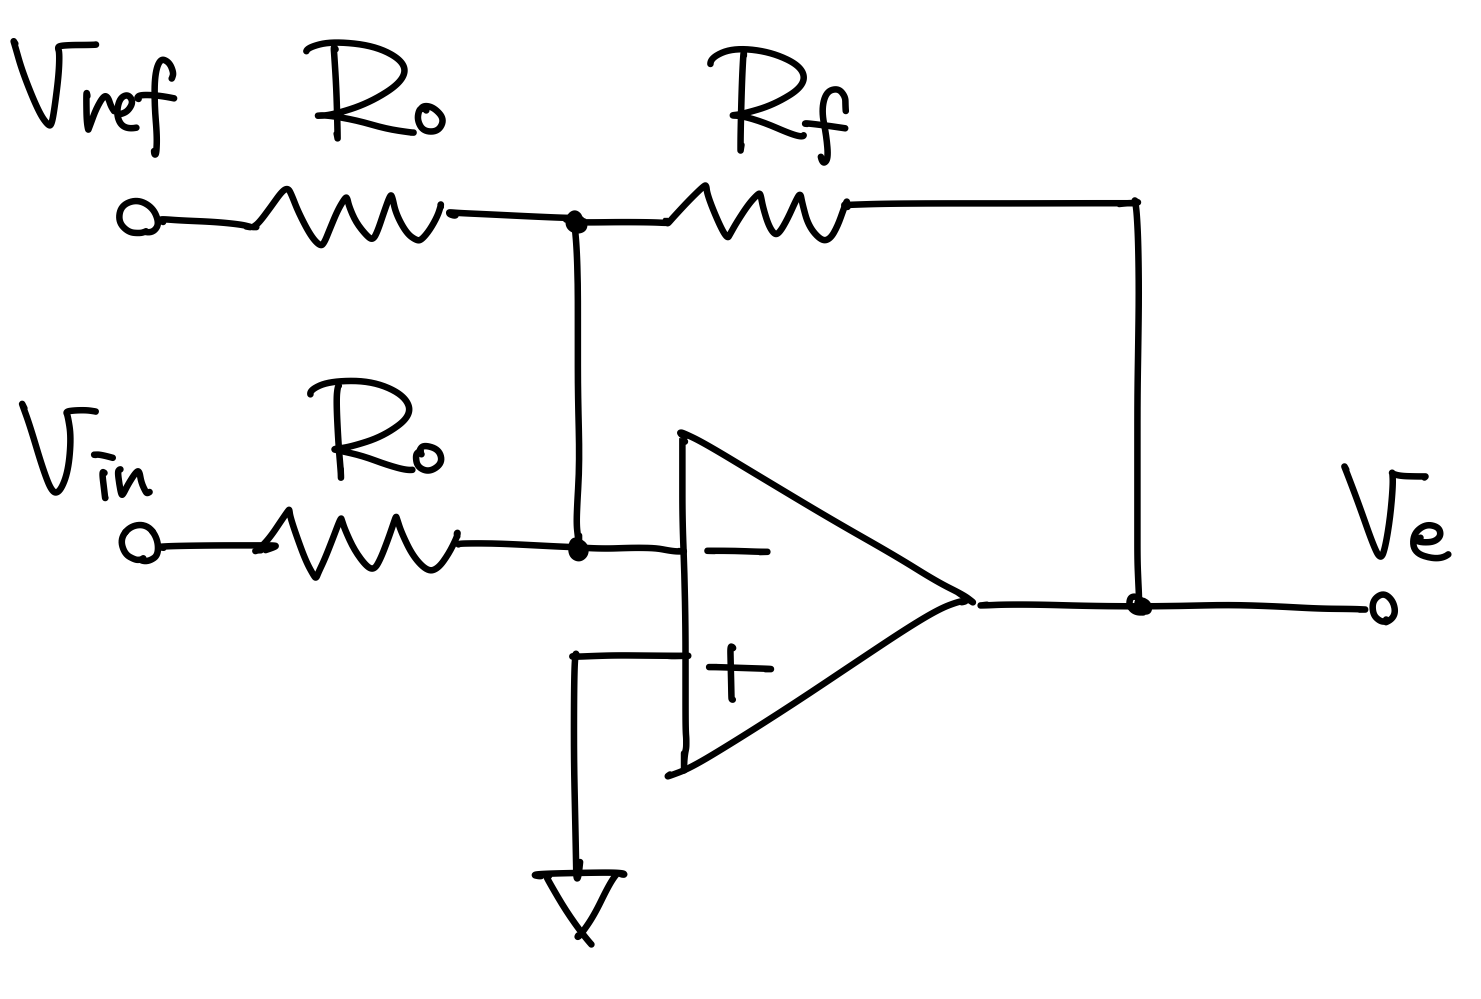
\includegraphics[width=0.8\columnwidth]{3_add.png}
          \caption{加算回路の概略図}\label{fig:3_add}
        \end{minipage}
        \begin{minipage}{0.45\columnwidth}
          \centering
          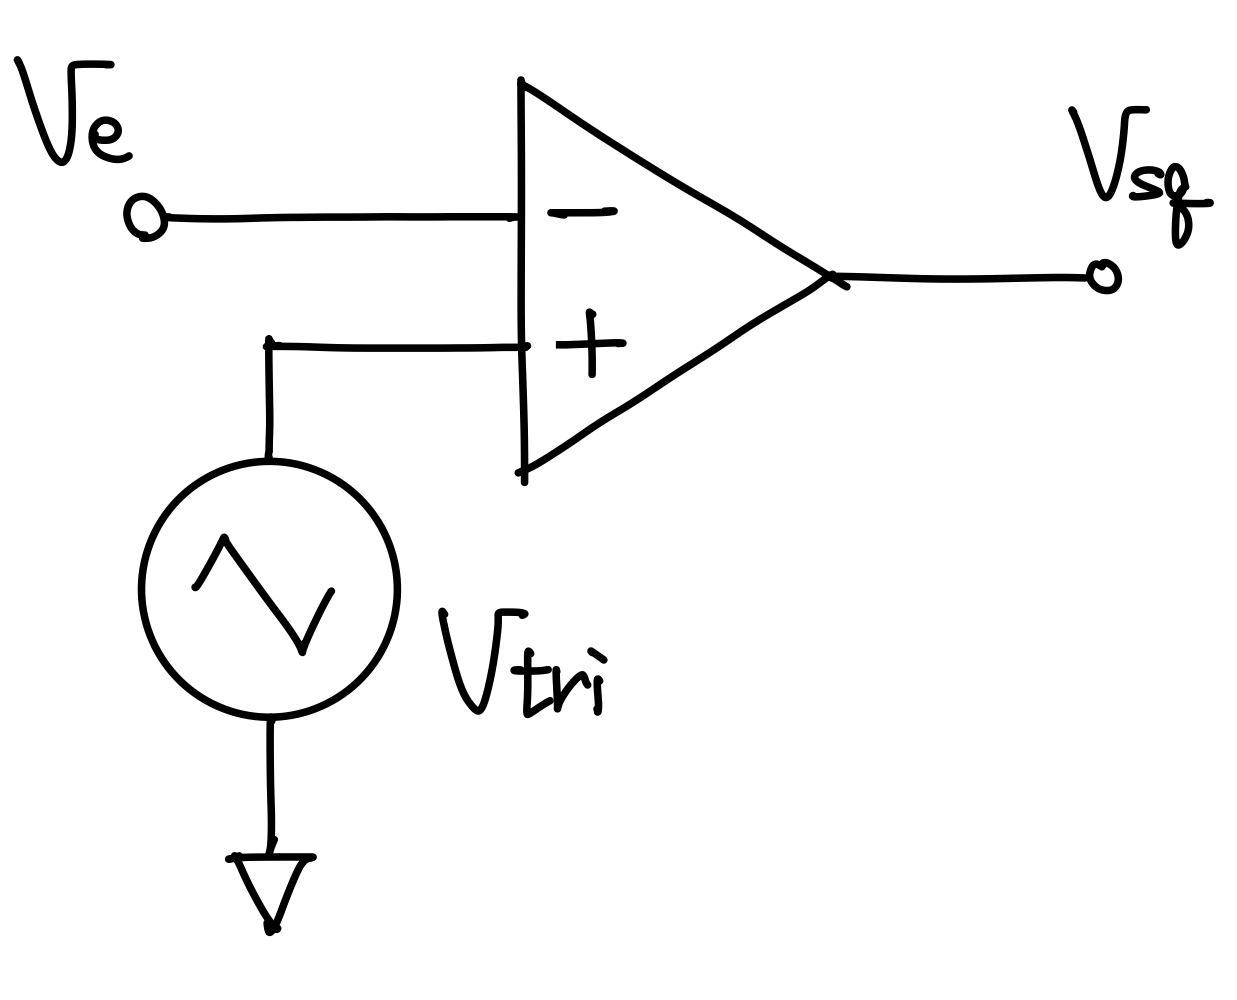
\includegraphics[width=0.8\columnwidth]{3_comp.png}
          \caption{比較回路の概略図}\label{fig:3_comp}
        \end{minipage}
      \end{figure}

    \subsubsection{フィードバック付きDCDCコンバータ}

      フィードバック付きDCDCコンバータの回路図を図\ref{fig:3_DCDC_add_comp}に示す.ここでは$V_\mathrm{in}$が表す電圧がこれまでと異なり,DCDCコンバータの入力電圧になることに注意されたい.図中のGは,DCDCコンバータ回路内のトランジスタのゲート端子を表す.


      \begin{figure}[htbp]
        \begin{center}
          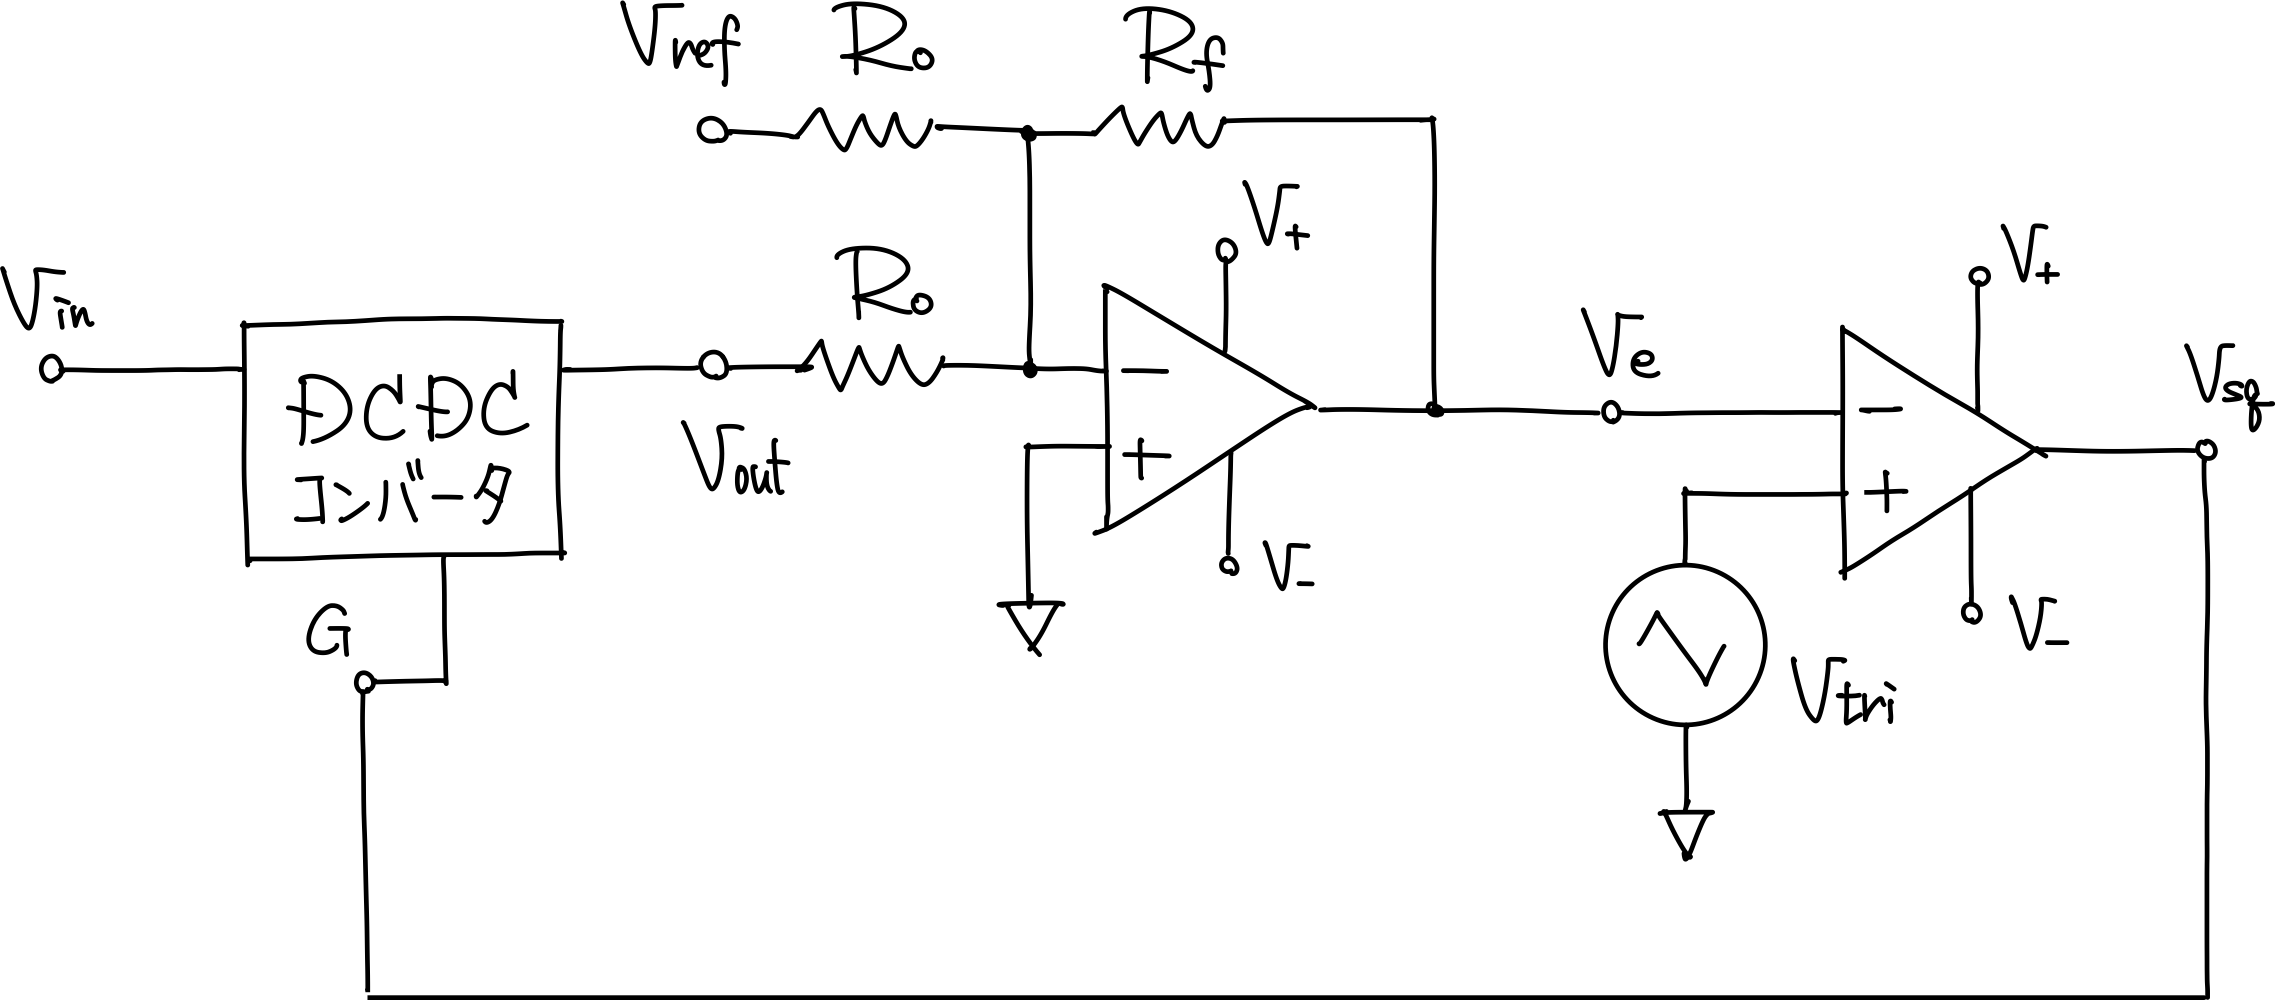
\includegraphics[width=0.8\columnwidth]{3_DCDC_add_comp.png}
          \caption{フィードバック付きDCDCコンバータ}\label{fig:3_DCDC_add_comp}
        \end{center}
      \end{figure}

      DCDCコンバータの入出力特性は

      \begin{equation}
        V_\mathrm{out} = -\frac{D}{1-D}V_\mathrm{in}
      \end{equation}
      であり,ここに式(\ref{eq:D})を代入して整理すると,

      \begin{equation}
        V_\mathrm{in} = - V_\mathrm{out} \cdot\frac{V_\mathrm{tri}-2K_\mathrm{fb}(V_\mathrm{ref}+V_\mathrm{out})}{V_\mathrm{tri}+2K_\mathrm{fb}(V_\mathrm{ref}+V_\mathrm{out})} \label{eq:3_DCDC_add_comp}
      \end{equation}
      という関係が成り立つ.これで,回路全体のパラメータを使って入出力特性を求めることができた.

  \subsection{方法}

    \subsubsection{実験1}

      図\ref{fig:3_add_comp_circ}に示す加算器と比較機を組み合わせた回路で,
      \begin{itemize}
        \item $R_0 = \SIs{10}{\kilo\ohm}$
        \item $V_\mathrm{ref} = \SIs{8.03}{\volt}$
        \item $V_\mathrm{tri} = \SIs{13}{\volt}$(peak-to-peak)
        \item (三角波の周波数) = $\SIs{50}{\kilo\hertz}$
        \item $V_+ = \SIs{15}{\volt}$
        \item $V_- = \SIs{-15}{\volt}$
      \end{itemize}
      とし,$K_\mathrm{fb} = -0.2, -0.51, -0.71$と変化させ,それぞれについて入力電圧$V_\mathrm{in}$と,方形波$V_\mathrm{sq}$のデューティ比$D$との関係を測定する.


      \begin{figure}[htbp]
        \begin{center}
          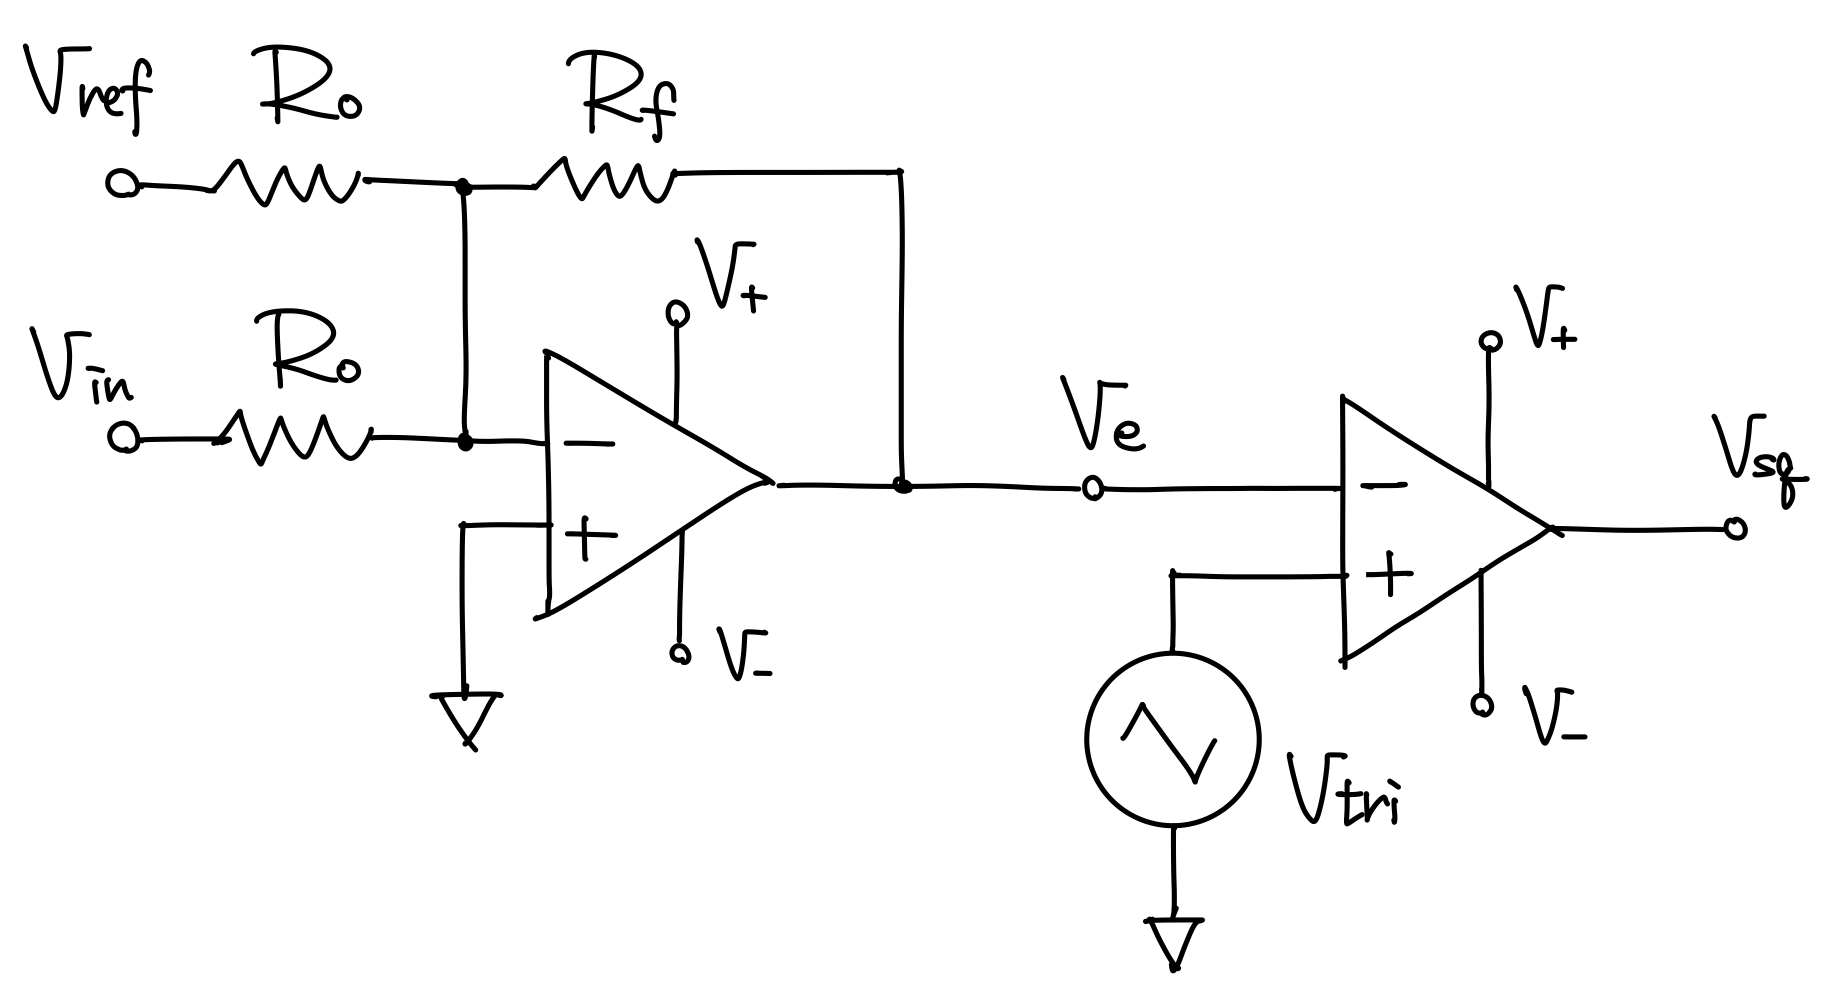
\includegraphics[width=0.8\columnwidth]{3_add_comp.png}
          \caption{実験1の回路図}\label{fig:3_add_comp_circ}
        \end{center}
      \end{figure}

    \subsubsection{実験2}

      測定対象の回路は図\ref{fig:3_DCDC_add_comp}で,実験1と同じパラメータで,$K_\mathrm{fb} = -0.2,-0.51$と変化させ,それぞれについて入力電圧と出力電圧とを測定する.

  \subsection{結果}

    \subsubsection{実験1}

      実験1の結果と,それぞれの理論線(式(\ref{eq:D}))を図\ref{fig:3_add_comp_result}に示す.

      \ref{fig:3_add_comp_result}からは,電圧が大きくなるにつれてデューティ比が直線的に大きくなることと,$K_\mathrm{fb}$が小さくなる(絶対値が大きくなる)につれてその直線の傾きが大きくなることが分かった.


      \begin{figure}[htbp]
        \begin{minipage}{0.45\columnwidth}
          \centering
          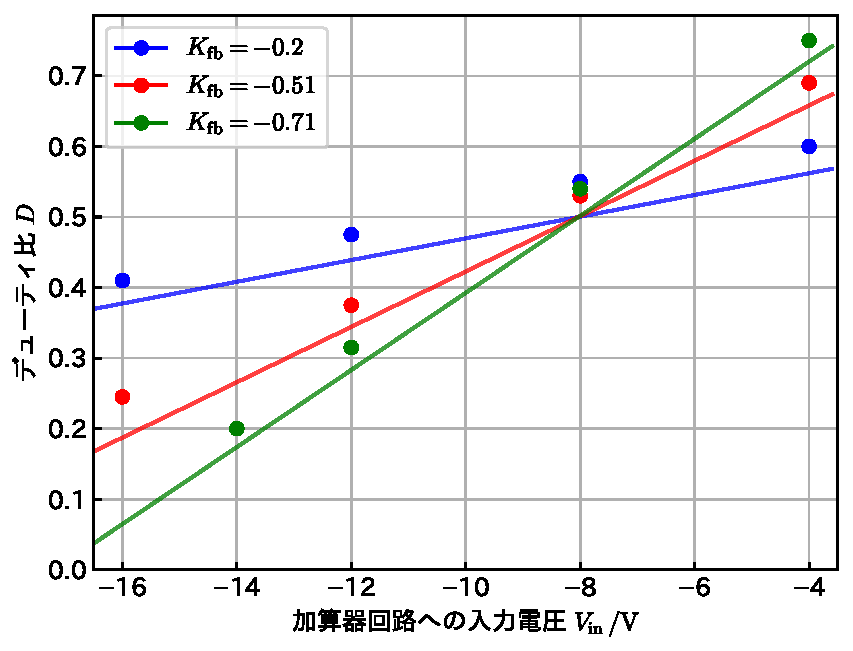
\includegraphics[width=0.8\columnwidth]{3_add_comp.pdf}
          \caption{実験1の結果}\label{fig:3_add_comp_result}
        \end{minipage}
        \begin{minipage}{0.45\columnwidth}
          \centering
          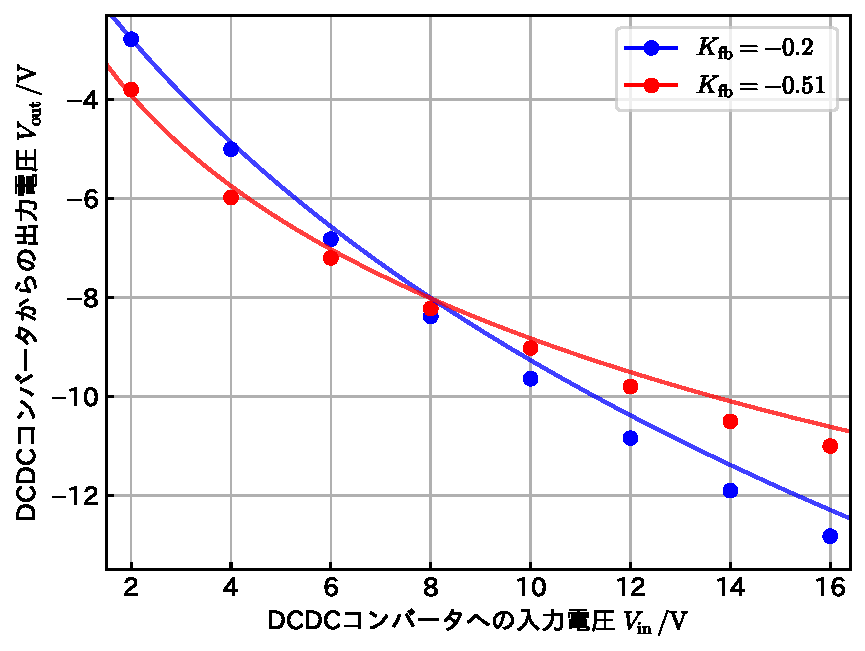
\includegraphics[width=0.8\columnwidth]{3_DCDC_add_comp.pdf}
          \caption{実験2の結果}\label{fig:3_DCDC_add_comp_result}
        \end{minipage}
      \end{figure}

    \subsubsection{実験2}

      実験2の結果とそれぞれの理論線(式\ref{eq:3_DCDC_add_comp})を図\ref{fig:3_DCDC_add_comp_result}に示す.

      $V_\mathrm{out}=\SIs{-8}{\volt}$付近を通る曲線の特性が見られ,また,$K_\mathrm{fb}$の絶対値が大きくなるほど曲線の傾きが小さくなることが観察できた.

  \subsection{考察}

    \subsubsection{実験1}

      図\ref{fig:3_add_comp_result}の測定点は理論線に沿って入るが,全体として理論値よりも大きい値であった.方形波を観察してみると図\ref{fig:oscillo}の紫色の線のような台形の波形が見られた.この波形の立ち上がり時間は$\SIs{10}{\text{\textmu}\second}$であり,これはオペアンプのスルーレートと一致していた.以上から,オペアンプのスルーレートによって方形波が\ruby{歪}{ひず}み,オン時間が長くなったことでデューティ比が大きくなったと考えられる.


      \begin{figure}[htbp]
        \begin{center}
          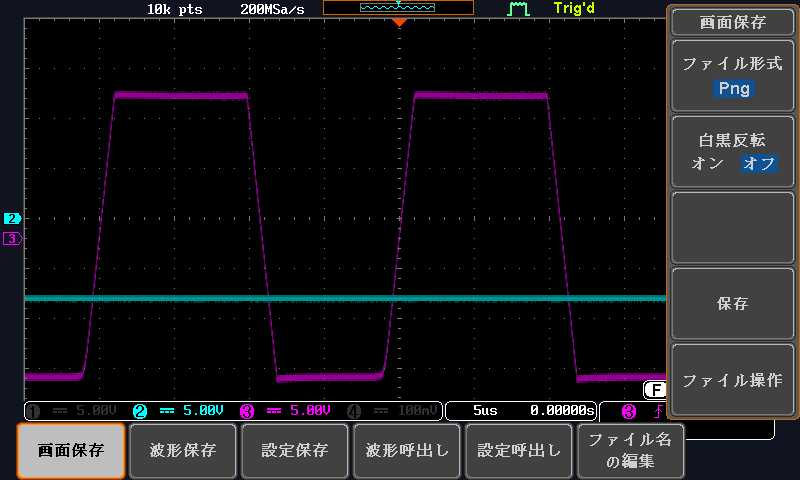
\includegraphics[width=0.5\columnwidth]{oscillo.jpg}
          \caption{$V_\mathrm{sq}$の波形}\label{fig:oscillo}
        \end{center}
      \end{figure}

    \subsubsection{実験2}
      実験1で述べたデューティ比の影響で,入力電圧が大きいところで出力電圧が理論値よりも大きくなっている.これを理論値に近づけるには,
      \begin{itemize}
        \item 周期に対してスルーレートが十分小さいような周波数域の三角波を利用する
        \item 加算器のフィードバック定数$K_\mathrm{fb}$の絶対値を大きくする
      \end{itemize}
      等が挙げられる.

\end{document}

% %!TEX root = 1_power_supply.tex
\documentclass[1_power_supply.tex]{subfiles}
\graphicpath{{../figures}}
\begin{document}

\section{電源システムの評価}

  \subsection{目的}

    これまでの実験で使った回路を組み合わせて,電源システム全体としての特性を評価する.

  \subsection{方法}

    電源システム全体を図\ref{fig:4_power_supply}に示す.


    \begin{figure}[htbp]
      \begin{center}
        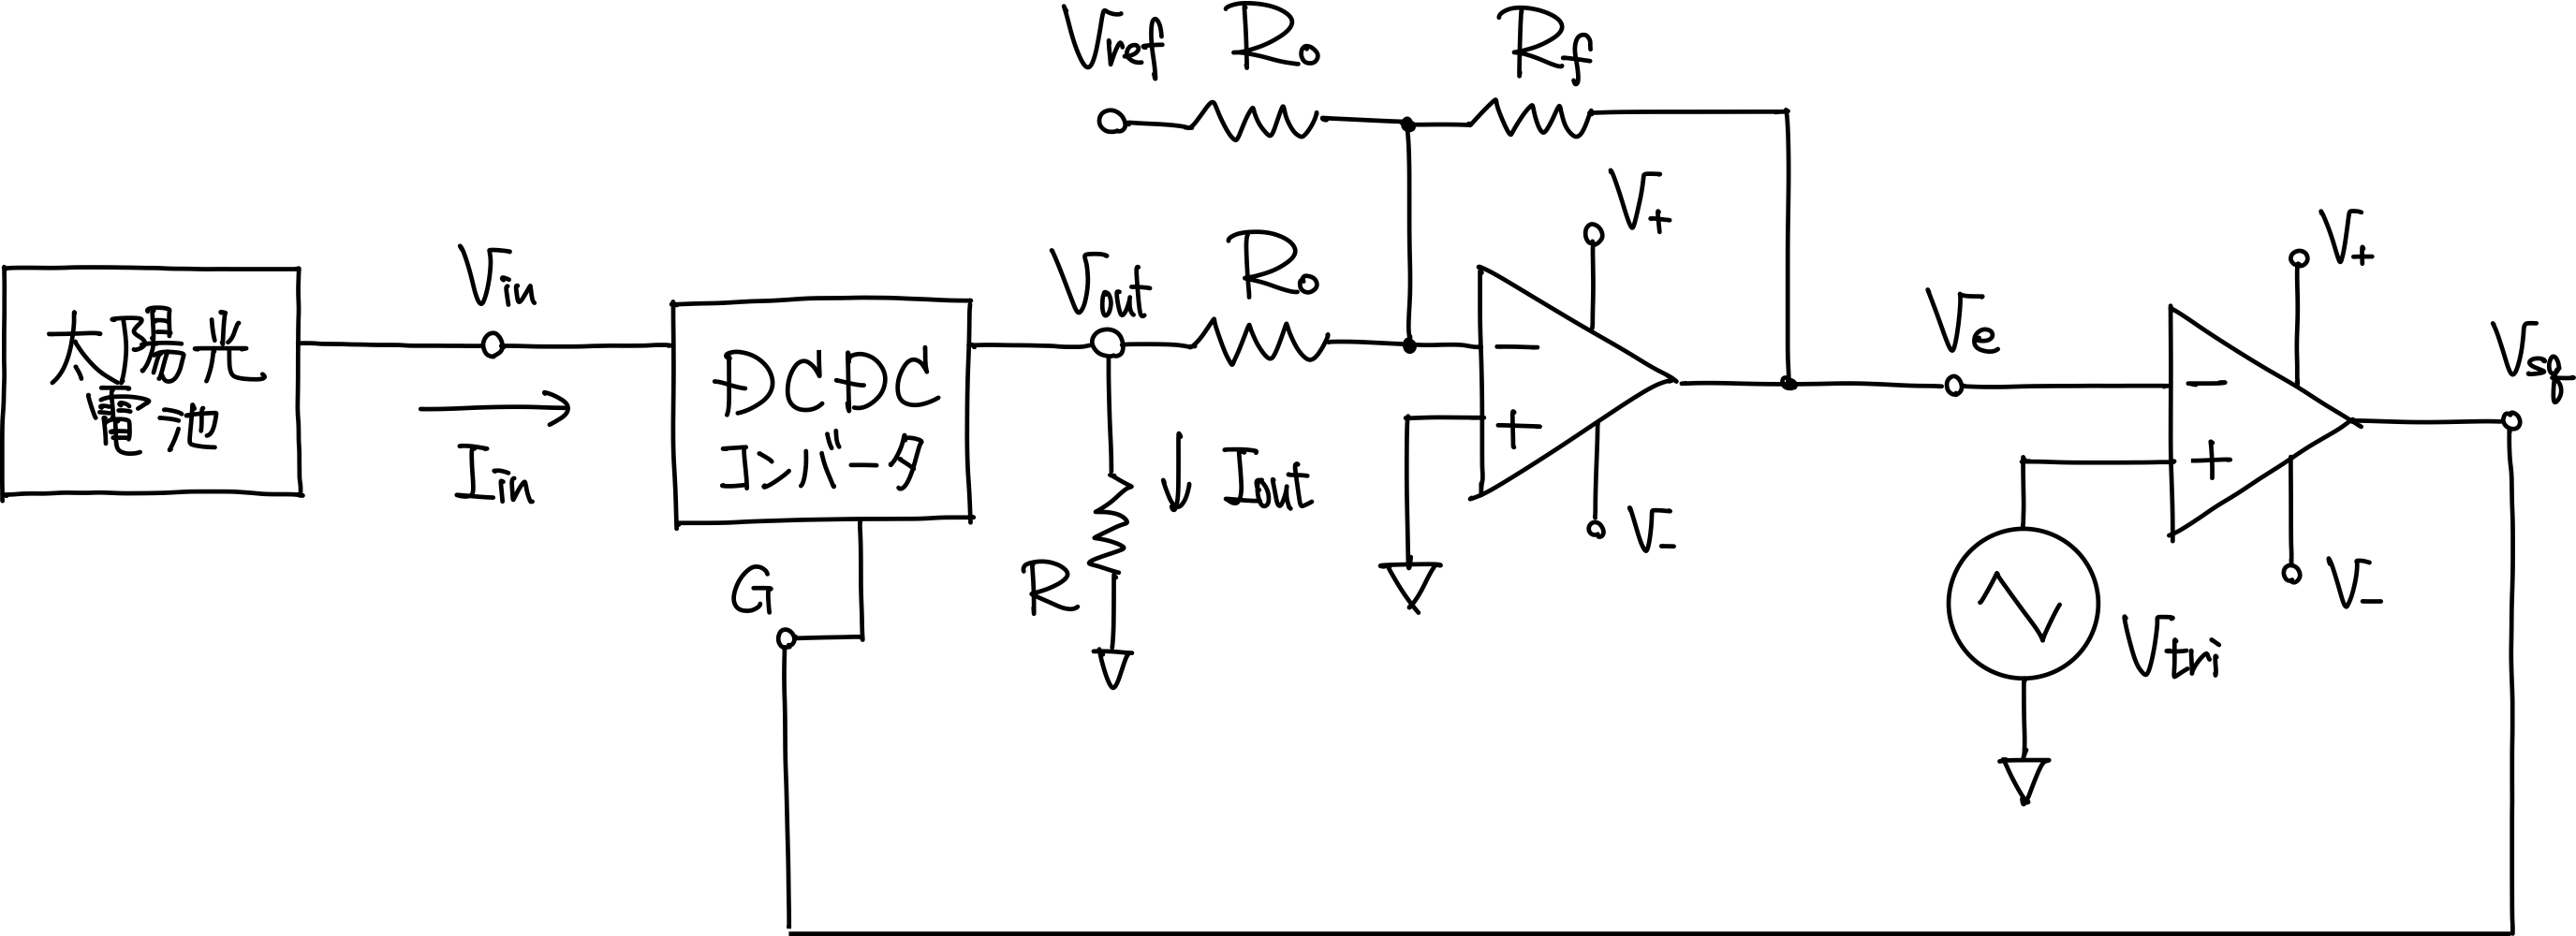
\includegraphics[width=0.8\columnwidth]{4_power_supply.png}
        \caption{電源システムの回路図}\label{fig:4_power_supply}
      \end{center}
    \end{figure}

    \begin{itemize}
      \item $R_0 = \SIs{2}{\kilo\ohm}$
      \item $R_\mathrm{f} = \SIs{10}{\kilo\ohm}$
      \item $V_\mathrm{tri} = \SIs{13}{\volt}$(peak-to-peak)
      \item (三角波の周波数) = $\SIs{50}{\kilo\hertz}$
      \item $V_+ = \SIs{15}{\volt}$
      \item $V_- = \SIs{-15}{\volt}$
    \end{itemize}
    と設定する.$R_0,R_\mathrm{f}$の値から分かるように,今回の測定では$K_\mathrm{fb}=-5$で固定とする.$\mathrm{AC}=\SIs{55.5}{\centi\meter},\SIs{85.5}{\centi\meter}$の場合で,$V_\mathrm{ref}$を変化させて入力電圧・電流,出力電圧・電流を測定する.

  \subsection{結果}

    目標電圧$V_\mathrm{ref}$と,入力電圧・電流,出力電圧・電流との関係を図\ref{fig:4_vin}-\ref{fig:4_iout}に示す.


    \begin{figure}[htbp]
      \centering
      \begin{minipage}{0.45\columnwidth}
        \centering
        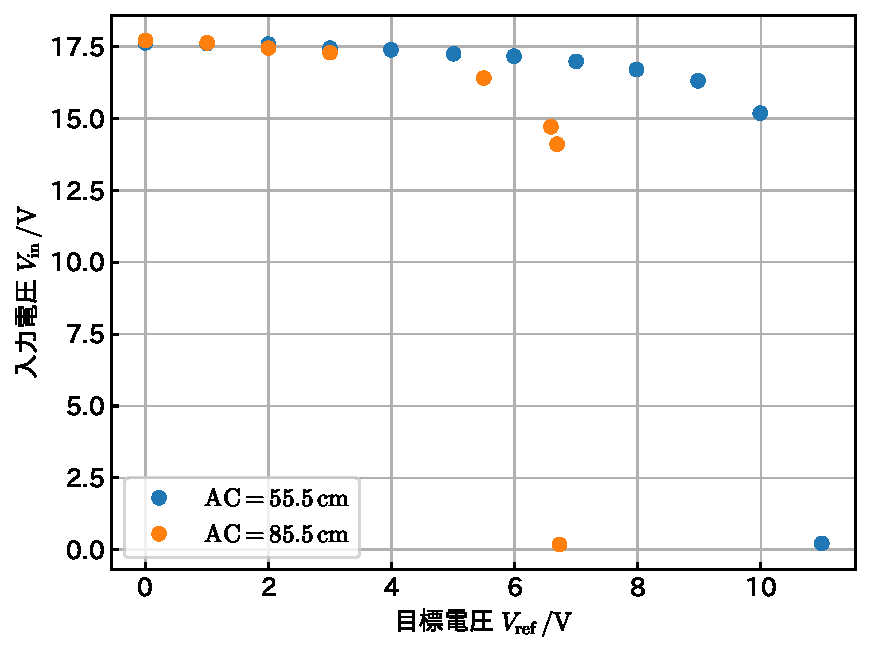
\includegraphics[width=0.8\columnwidth]{4_-5_vin.pdf}
        \subcaption{入力電圧}\label{fig:4_vin}
      \end{minipage}
      \begin{minipage}{0.45\columnwidth}
        \centering
        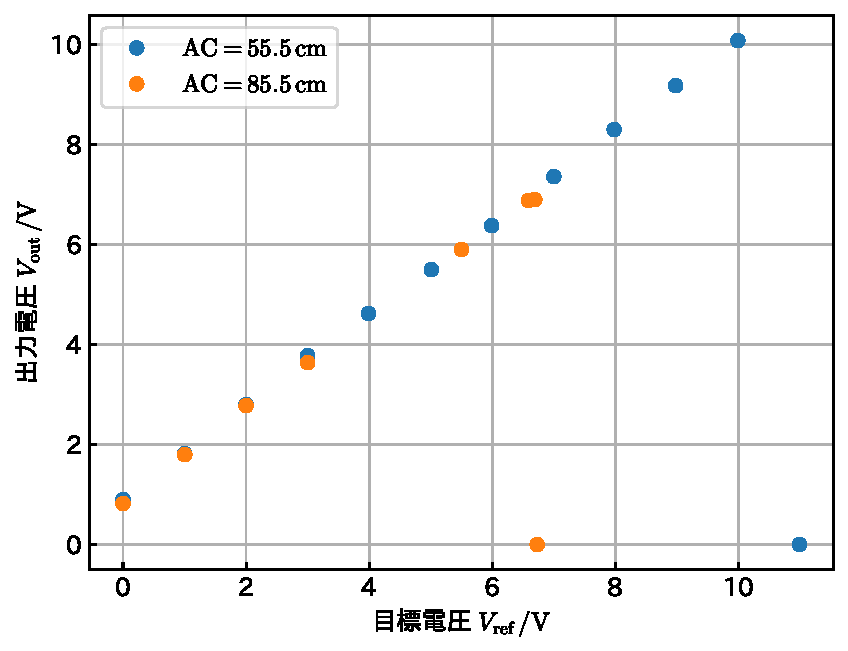
\includegraphics[width=0.8\columnwidth]{4_-5_vout.pdf}
        \subcaption{出力電圧}\label{fig:4_vout}
      \end{minipage}
      \hspace{5mm}
      \begin{minipage}{0.45\columnwidth}
        \centering
        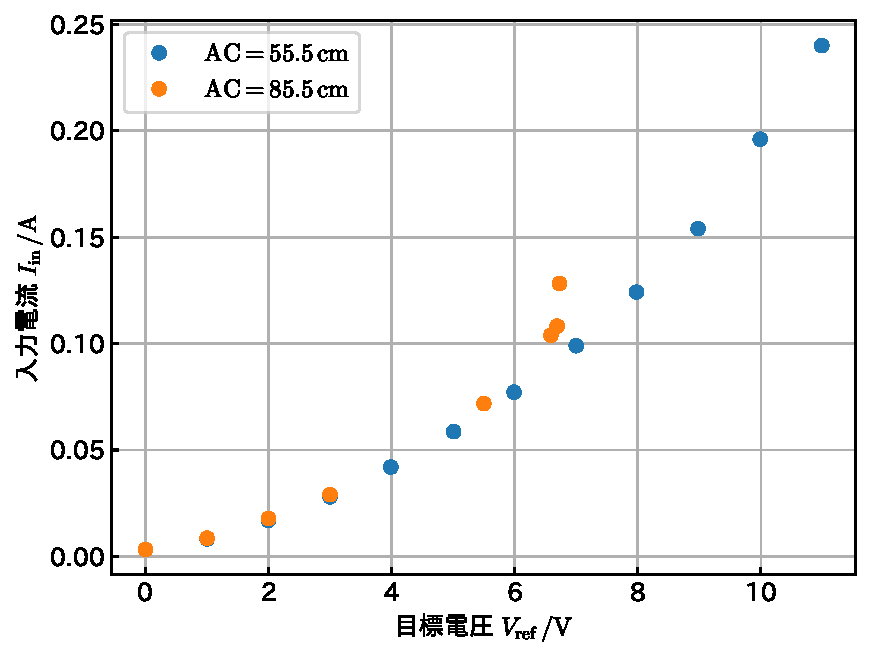
\includegraphics[width=0.8\columnwidth]{4_-5_iin.pdf}
        \subcaption{入力電流}\label{fig:4_iin}
      \end{minipage}
      \begin{minipage}{0.45\columnwidth}
        \centering
        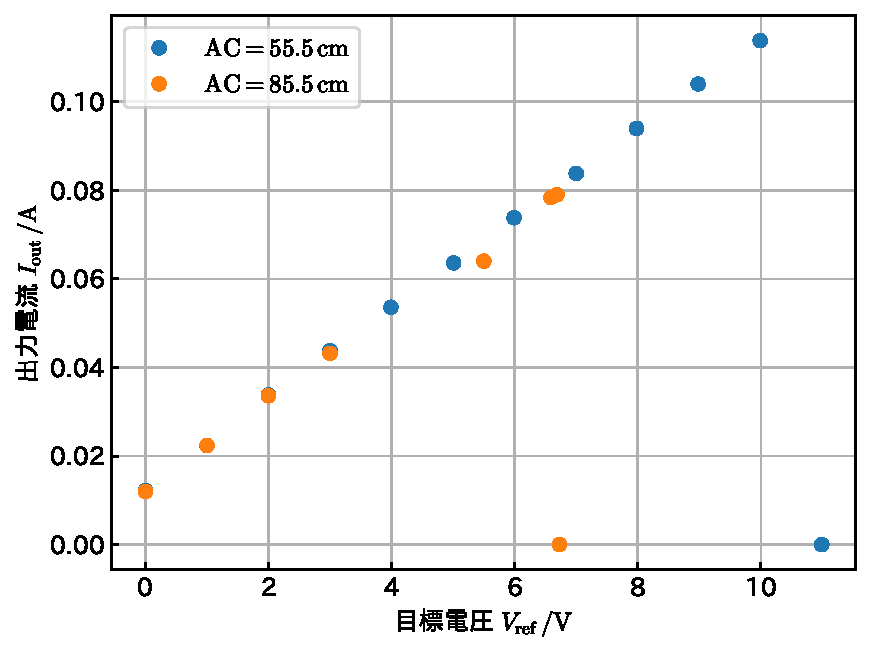
\includegraphics[width=0.8\columnwidth]{4_-5_iout.pdf}
        \subcaption{出力電流}\label{fig:4_iout}
      \end{minipage}
      \caption{各測定の結果}
      \label{figs:4_result}
    \end{figure}
    $\mathrm{AC}=\SIs{55.5}{\centi\meter}$のときは$V_\mathrm{ref}=\SIs{11}{\volt}$,$\mathrm{AC}=\SIs{85.5}{\centi\meter}$のときは$V_\mathrm{ref}=\SIs{6.7}{\volt}$で大きく測定値が変化していることがわかる.

  \subsection{考察}

    入力電流・電圧,出力電流・電圧からそれぞれ入力電力,出力電力を計算しプロットしたものをそれぞれ\ref{fig:4_pin},\ref{fig:4_pout}に,電力効率をプロットしたものを\ref{fig:4_eff}に示す.


    \begin{figure}[htbp]
      \centering
      \begin{minipage}{0.45\columnwidth}
        \centering
        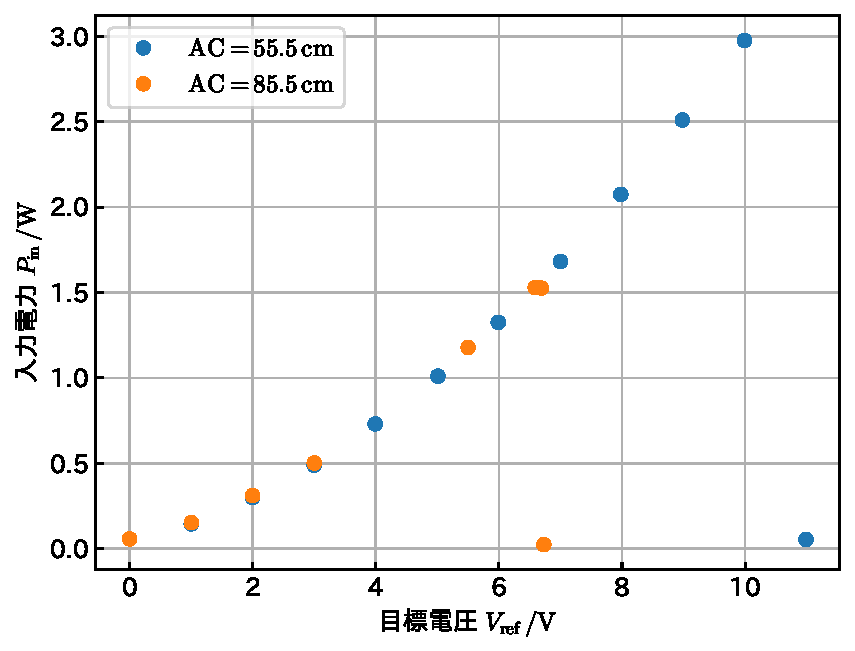
\includegraphics[width=0.8\columnwidth]{4_-5_pin.pdf}
        \subcaption{入力電力}\label{fig:4_pin}
      \end{minipage}
      \begin{minipage}{0.45\columnwidth}
        \centering
        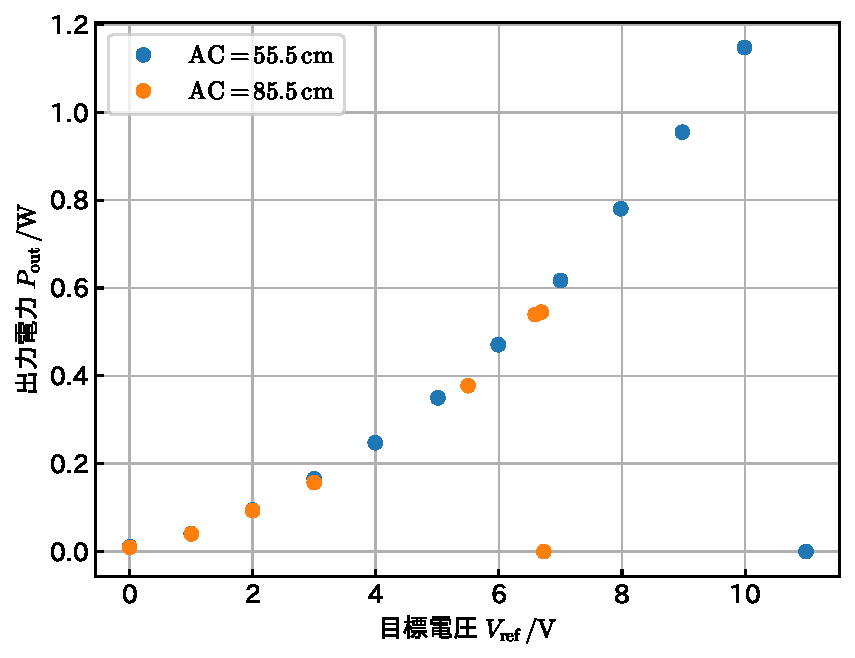
\includegraphics[width=0.8\columnwidth]{4_-5_pout.pdf}
        \subcaption{出力電力}\label{fig:4_pout}
      \end{minipage}
      \hspace{5mm}
      \begin{minipage}{\columnwidth}
        \centering
        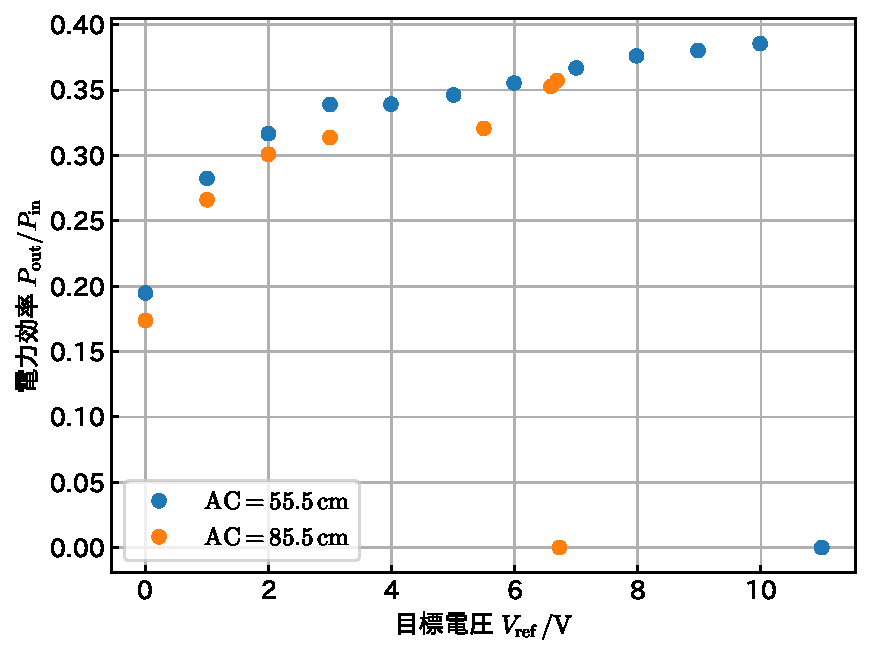
\includegraphics[width=0.8\columnwidth]{4_-5_eff.pdf}
        \subcaption{電力効率}\label{fig:4_eff}
      \end{minipage}
      \caption{電力のプロット}
      \label{figs:4_think}
    \end{figure}


    \begin{figure}[htbp]
      \begin{center}
        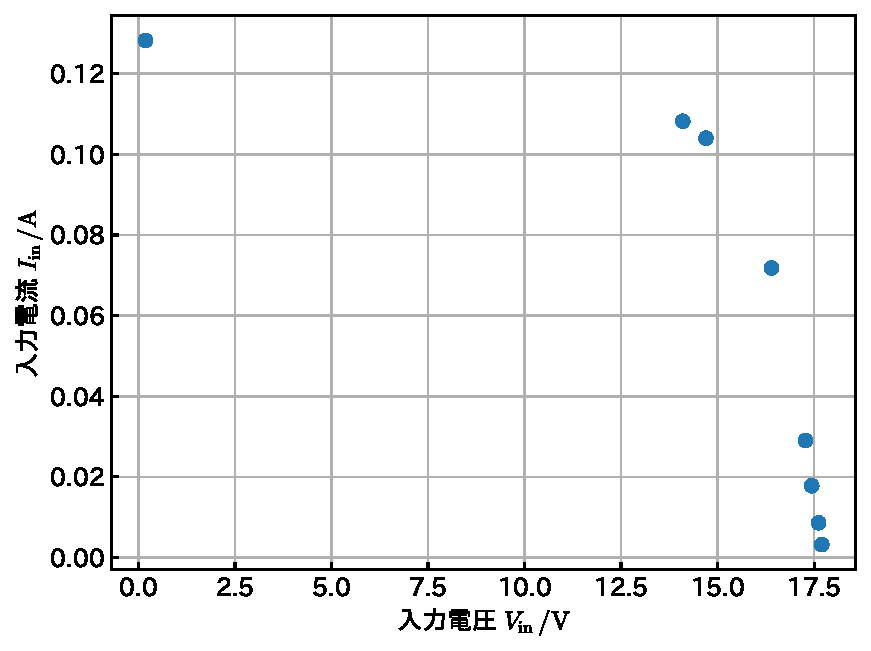
\includegraphics[width=0.8\columnwidth]{4_-5_90_vi.pdf}
        \caption{入力の電圧-電流特性($\mathrm{AC}=\SIs{85.5}{\centi\meter}$)}\label{fig:4_v-i}
      \end{center}
    \end{figure}

    電力効率は,目標電圧が0である点と測定点が大きく変化する点を除いて$\SIs{25}{\percent}\sim\SIs{40}{\percent}$となった.なお,入力の電流・電圧特性は図\ref{fig:4_v-i}に示すとおりで,$(V_\mathrm{in},I_\mathrm{in})=(\SIs{6.90}{\volt}, \SIs{0.0790}{\ampere})$のときに最大電力で動作することが分かる.

    また,測定点が大きく変化した(途切れた)点の原因については,差信号$V_\mathrm{e}$が三角波の振幅よりも大きくなり,デューティ比が1になったからと考える.

\end{document}


\subfile{1_power_supply_1.tex}
\clearpage
\subfile{1_power_supply_2.tex}
% \clearpage
% \subfile{1_power_supply_3.tex}
% \clearpage
% \subfile{1_power_supply_4.tex}

\end{document}